\documentclass[
    iai, % Saisir le nom de l'institut rattaché
    il, % Saisir le nom de l'orientation
]{heig-tb}

\usepackage[nooldvoltagedirection,european,americaninductors]{circuitikz}
\usepackage{graphicx}
\graphicspath{ {./assets/figures/} }

\signature{signature.svg}

\makenomenclature
\makenoidxglossaries
\makeindex

\addbibresource{bibliography.bib}

\usepackage{etoolbox}
\renewcommand\nomgroup[1]{%
  \item[\bfseries
  \ifstrequal{#1}{A}{Constantes physiques}{%
  \ifstrequal{#1}{B}{Groupes}{%
  \ifstrequal{#1}{C}{Autres Symboles}{}}}%
]}

\newcommand{\nomunit}[1]{%
\renewcommand{\nomentryend}{\hspace*{\fill}#1}}

\nomenclature[A, 02]{\(c\)}{\href{https://physics.nist.gov/cgi-bin/cuu/Value?c}
{Vitesse de la lumière dans le vide}
\nomunit{\SI{299792458}{\meter\per\second}}}

\nomenclature[A, 03]{\(h\)}{\href{https://physics.nist.gov/cgi-bin/cuu/Value?h}
{Constante de Planck}
\nomunit{\SI[group-digits=false]{6.62607015e-34}{\joule\per\hertz}}}

\nomenclature[A, 01]{\(G\)}{\href{https://physics.nist.gov/cgi-bin/cuu/Value?bg}
{Constante de gravitation universelle}
\nomunit{\SI[group-digits=false]{6.67430e-11}{\meter\cubed\per\kilogram\per\second\squared}}}

\nomenclature[B, 03]{\(\mathbb{R}\)}{Nombres réels}
\nomenclature[B, 02]{\(\mathbb{C}\)}{Nombres complexes}
\nomenclature[B, 01]{\(\mathbb{H}\)}{Quaternions}

\nomenclature[C]{\(V\)}{Volume constant}
\nomenclature[C]{\(\rho\)}{Indice de frottement sec}

\newacronym{gcd}{GCD}{Plus grand diviseur commun}
\newacronym{lcm}{LCM}{Plus petit multiple commun}

\newglossaryentry{heig-vd}{
    name=HEIG-VD,
    description={Haute École d'Ingénierie et de Gestion du canton de Vaud}
}

\newglossaryentry{uml}{
    name=UML,
    description={Notation pour la modélisation d'applications en ingénieurie logiciel}
}

\newglossaryentry{diagrams}{
    name=diagrams.net,
    description={Site web permettant de créer des diagrammes}
}

\newglossaryentry{websig}{
    name=webSIG,
    description={systèmes d'interface web de visualisation de données géographiques}
}

\newglossaryentry{epfl}{
name=EPFL
description={Ecole polytechnique fédéral de Lausanne}
}
% Auteur du document (étudiant-e) en projet de Bachelor
\author{Kylian Bourcoud}

% Activer l'option pour l'accord du féminin dans le texte
%\genre{female}

% Titre de votre travail de Bachelor
\title{Plans de la HEIG-VD interactifs}

% Le sous titre est optionnel
\subtitle{Travail de Bachelor}

% Nom du professeur responsable
\teacher {Prof. Y. Chevallier (HEIG-VD)}

% Mettre à jour avec la date de rendu du travail
\date{\today}

% Numéro de TB
\thesis{7212}



\surroundwithmdframed{minted}

\setcounter{tocdepth}{1}

%% Début du document
\begin{document}
\selectlanguage{french}
\maketitle
\frontmatter
\clearemptydoublepage

%% Requis par les dispositions générales des travaux de Bachelor
\preamble
\authentification

%% Résumé / Version abbrégée
\begin{abstract}
    % Francais
Ce rapport décrit le processus de création d'une application web de plans interactifs pour la HEIG-VD.
Ce processus est séparé en cinq étape : une introduction au contexte,
une analyse des besoins des utilisateurs et des sytèmes déja existentes,
la conception d'une solution, la réalisation de celle-ci,
et finalement une critique du travail accompli.



\asterism

% English
This report describes the creation process for a web application of interactive plan for the HEIG-VD school.
This process is separated in five steps : an introduction of the context,
an analysis of the users needs and the existants solutions,
the conception of a solution, the development
and finally a review of the accomplished work.
\end{abstract}

%% Sommaire et tables
\clearemptydoublepage
{
    \tableofcontents
    \let\cleardoublepage\clearpage
    \listoffigures
    \let\cleardoublepage\clearpage
    \listoftables
    %\let\cleardoublepage\clearpage
    %\listoflistings
}

\printnomenclature
\clearemptydoublepage
\pagenumbering{arabic}

%% Contenu
\mainmatter
\chapter{Introduction}
\section{Contexte}
Les cartes qu'elle soit schématique ou précise ont été un outil très utile pour l'orientation des personnes au sein d'une région ou d'un bâtiment.
Avec l'arrivée du web, l'usage des plateformes de cartes comme google maps ont peu à peu remplacer les cartes papier, amenant des fonctionnalités plus interactives.

\begin{figure}[h]
    \centering
    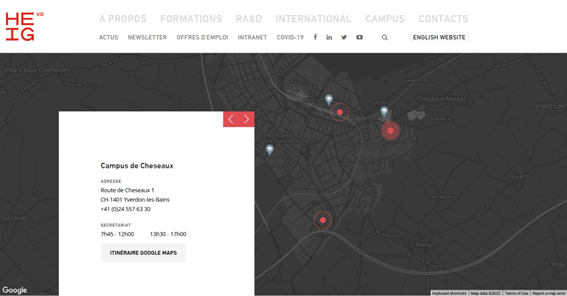
\includegraphics{actual_heig_plan.png}
    \caption{Plans actuels de la HEIG-VD}
    \label{fig:heigCurrentMap}
\end{figure}

La \gls{heig-vd} est une haute école dispensant des formations dans différents domaines de l'ingénieurie, ainsi que de la gestion d'entreprise.
Elle se situe sur trois sites dispersé dans la ville d'Yverdon-Les-Bains
: Cheseaux  situé en périphérie de la ville, St-Roch situé proche de la gare et le Y-Parc situé dans la zone industrielle.

Cette école fournit, sur son site web un plan \cite{plan-heig} (voir Figure \ref{fig:heigCurrentMap}) indiquant l'emplacement des trois bâtiments pricipaux.
On peut aussi y obtenir les informations sur les différents moyens d'accès à ces sites afin d'aider ses utilisateurs à s'orienter.
Cependant elle ne fournit, ni sur son site, ni dans le guide de l'étudiant, une interface permettant de s'orienter vers une salle ou une ressource précise.

\section{Description du problème}
M.Chevallier souhaite mettre à disposition aux utilisateurs une interface interactive pour visualiser les salles et les plans de la \gls{heig-vd} pour les trois bâtiments.

\chapter{Analyse}
\section{Analyse fonctionnelle du système}
L'analyse fonctionnelle est un processus qui permets de déterminer les fonctionnalités d'un système à partir d'une analyse des besoins utilisateurs.

\subsection{Cas d'utilisation}
La première étape est de déterminer les cas d'utilisations du futur système.
Ceux-ci ont été établi lors de la conception du schéma des cas d'utilisation, figure \ref{useCaseDiagram.drawio.pdf}.
Celui-ci est en notation \gls{uml}, un des standards utilisé dans la modélisation d'application logiciel,
et a été réalisé à l'aide de l'application web \gls{diagrams} \cite{diagrams}.

\fig[width=7cm]{Schéma des cas d'utilisations}{useCaseDiagram.drawio.pdf}

\newpage
Ce schéma présente les cas d'utilisation suivant :
\begin{itemize}
    \item Un utilisateur utilise le système pour s'orienter sur les différents sites de la HEIG-VD.
    \item Un utilisateur opère une recherche sur le système afin de localiser une ressource par des critères ou par son nom (une ressource est un terme générique pouvant symboliser une salle, l'emplacement d'un bureau d'un collaborateur, l'emplacement de matériel, etc.).
    \item Un utilisateur obtient des informations sur une ressource.
    \item Un utilisateur personnalise la carte et l'exporte pour d'autre usage.
\end{itemize}

\subsection{Analyse des besoins}
La deuxième étape de l'analyse fonctionnelle est de déterminer les besoins des utilisateurs à partir des cas d'utilisation du système.
Pour ce système les besoins ont été déterminé dans le tableau \ref{besoins}. Ils ont été numérotés de N1 à N8 pour pouvoir s'y référer plus facilement par la suite.
\begin{table}[h]
    \begin{center}
        \caption{Liste des Besoins \label{besoins}}
        \begin{tabular}{l|l}
               & Besoin                                                                  \\ \hline
            N1 & S'orienter facilement à travers les sites de la HEIG-VD                 \\
            N2 & Localiser une ressource à l'aide de son nom                             \\
            N3 & Localiser une ressource à l'aide de critères                            \\
            N4 & S'informer efficacement sur une ressource                               \\
            N5 & Être capable de personnaliser une carte                                 \\
            N6 & Être capable de partager sa carte personnalisée                         \\
            N7 & S'informer efficacement des noms des locaux, leur surface, et leur type \\
            N8 & Localiser facilement un collaborateur sur un plan des sites
        \end{tabular}
    \end{center}
\end{table}

\newpage

\subsection{fonctionnalités du système}
La troisième étape est de déterminer les fonctionnalités du système à partir des besoins des utilisateurs.
Ils ont été listés dans le tableau \ref{fonctions}.
De plus les besoins auxquelles ils répondent, ont été précisé dans la Besoin colonne du tableau.
\begin{table}[h]
    \begin{center}
        \caption{Liste des Fonctionnalités \label{fonctions}}
        \begin{tabular}{l|l|l}
                & Fonctionnalités                                                      & Besoin   \\ \hline
            F1  & Afficher un plan afin d'aider l'orientation                          & N1 N7    \\
            F2  & Utilisable facilement et de façon ergonomique                        & N1       \\
            F3  & Fournir une orientation rapidement                                   & N1       \\
            F4  & Facilement accessible                                                & N1       \\
            F5  & Afficher les ressources désirées                                     & N1 N3 N5 \\
            F6  & Fournir un outil de tracé de plus cour itinéraire pour l'orientation & N1       \\
            F7  & Offrir un outil de localisation de ressource par nom                 & N2 N8    \\
            F8  & Fournir un outil de localisation de ressource par critères           & N3       \\
            F9  & Fournir des informations sur les ressources                          & N4 N7    \\
            F10 & Fournir un outil de dessin sur carte                                 & N5       \\
            F11 & Fournir un outil d'exportation                                       & N5       \\
            F12 & Fournir un outil d'impression de carte                               & N6       \\
            F13 & Fournir un outil de partage de carte                                 & N6       \\
            F14 & Fournir un outil de sauvegarde de carte                              & N6
        \end{tabular}
    \end{center}
\end{table}

\section{Etat de l'art \Gls{websig}}
Dans cette section, différents systèmes d'interface web de visualisation de données géographiques (\gls{websig}) vont être analysés, ainsi que les technologies
associé à ce type d'application.

\subsection{\Gls{websig} existants}

\subsubsection{Plan EPFL}
\begin{figure}[h]
    \centering
    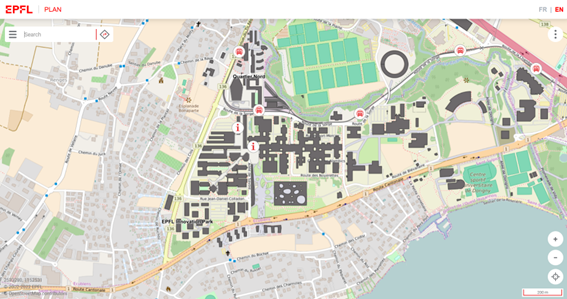
\includegraphics[scale=0.7]{planEPFL.png}
    \caption{Plans interactifs de l'EPFL}
\end{figure}

\textbf{Fonctionnalités}

Les plans interactifs du campus de l'\gls{epfl} \cite{plan-epfl} affichent les bâtiments du campus en s'adaptant selon le zoom et l'étage sélectionné.
Suivant le zoom on peut visualiser le contour du site, puis le contour des bâtiments et enfin les salles des bâtiments (voir \ref{fig:EPFLZoom})

\begin{figure}[h]
    \centering
    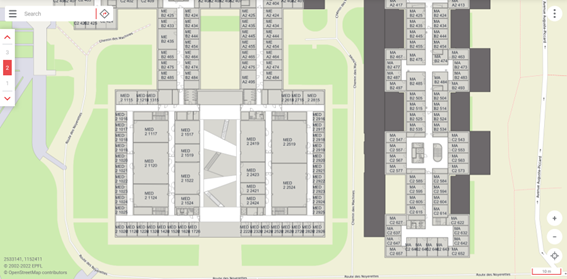
\includegraphics[scale=0.7]{planEPFLGrosPlan.png}
    \caption{Zoom sur les plans de l'EPFL }
    \label{fig:EPFLZoom}
\end{figure}

L'utilisateur a la possibilité de filtrer les points d'intérêts à afficher sur la carte à l'aide d'un menu sur la gauche du site.
Il y a aussi la possibilité de rechercher différentes ressources en fonction de leur nom comme les bâtiments, les salles, les personnes, les restaurant, les magasins, ou encore les espaces culturels.
D'autres outils sont fournis comme la recherche d'un plus court itinéraire entre deux ressources, un outil pour l'impression, ou encore changer l'affichage pour une vue aérienne.
Finalement un lien permet d'accéder au Géoportail de l'EPFL.

\textbf{Technologies utilisées}

La principale technologie utilisée pour le frontend est Ngeo (combine Angular js et openlayers, plus de détails dans la section technologie ).

\subsubsection{Géoportail EPFL}

\begin{figure}[h]
    \centering
    \includegraphics[scale=0.7]{géoportailEPFL.png}
    \caption{Géoportail de L'EPFL}
\end{figure}

Le Géoportail de l'EPFL \cite{geoportail-epfl} est très similaire au plan du campus, mais il offre la possibilité de dessiner des formes vectorielles sur la carte.
Il permet aussi d'afficher des ressources plus précises comme les réseaux wifi ou les prises électrique.

\subsubsection{MIT campus map}

\begin{figure}[h]
    \centering
    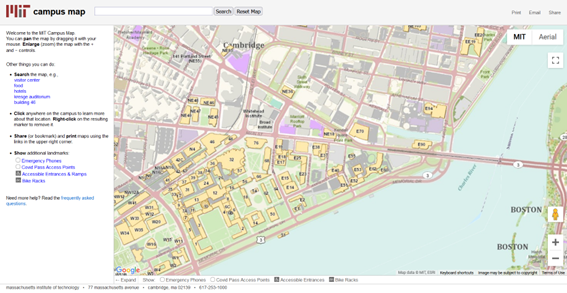
\includegraphics[scale=0.7]{MitCampusMap.png}
    \caption{carte du campus du MIT}
\end{figure}

\textbf{Fonctionnalités}

Le plan interactif du MIT \cite{mit-map} affiche le tracé des bâtiments ainsi que le nom de ceux-ci. Seulement les légendes s'adaptent en fonction du zoom.

Un utilisateur peut rechercher des bâtiments ou des points d'intérêts lié à l'université (ex : le world wide web consortium W3C).

Il peut aussi appliquer quelques filtres pour afficher des repères comme les restaurants. Cliquer sur un bâtiment permet d'obtenir des informations sur celui-ci. D'autres outils sont fournis comme un outil de partage ou d'impressions.

\textbf{Technologies utilisées}

L'affichage de la carte s'effectue à l'aide de l'api google maps. Ceci permet aussi un accès à google street view.

\subsubsection{SITN - Géoportail du système d'informations du territoire neuchâtelois}

\begin{figure}[h]
    \centering
    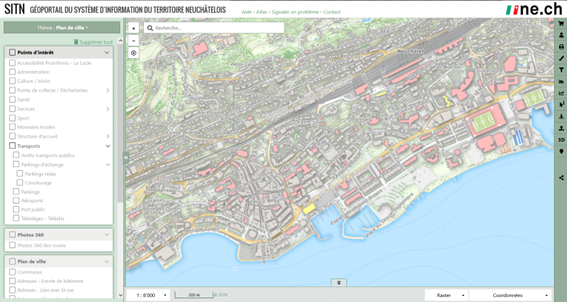
\includegraphics[scale=0.7]{planSITN.png}
    \caption{Plan du SITN}
\end{figure}

\textbf{Fonctionnalités}

Les plans du SITN \cite{sitn} affichent les différentes informations géographiques du canton de Neuchâtel.
Le niveau de détail de la carte s'adapte en fonction du zoom.
Par exemple les numéros des maisons selon le cadastre de chaque commune s'affichent lors d'un zoom à une échelle 1 :1000.

Il y a la possibilité d'appliquer plusieurs filtres afin d'obtenir les informations recherchées comme le tracé des commune ou les points d'intérêts.

L'outil offre aussi des outils de dessin vectoriel, d'impression, la possibilité de changer le fond du plan de changer un accès à google street map, et un accès au géoportail LIDAR

\textbf{Technologies utilisées}

Le site utilise GeoMapfish pour l'affichage des cartes ainsi que l'api google maps pour google street view.

\subsubsection{Standford Campus Map}

\begin{figure}[h]
    \centering
    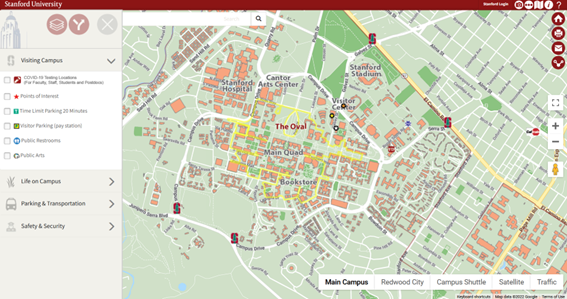
\includegraphics[scale=0.7]{standfordCampusMap.png}
    \caption{plan du campus de Standford}
\end{figure}

\textbf{Fonctionnalités}

Le carte du campus de Standford \cite{standford-map} affiche le tracé des bâtiments ainsi qu'une légende précisant le nom de ceux-ci.
Seul l'affichage de la légende varie selon le zoom : affiche seulement les légendes lors d'un affichage rapproché sur les bâtiments.

Le site offre un outil de recherche de ressources aux utilisateurs, un accès à open street view, un outil d'impression et un outil de partages.

A noter que le menu en bas à droite est un mélange de plusieurs fonctionnalités ce qui peut perdre un nouvel utilisateur.

\textbf{Technologies utilisées}

L'application web utilise l'api google maps pour l'affichage de la carte.

\subsubsection{Aéroport de Zürich}

\begin{figure}[h]
    \centering
    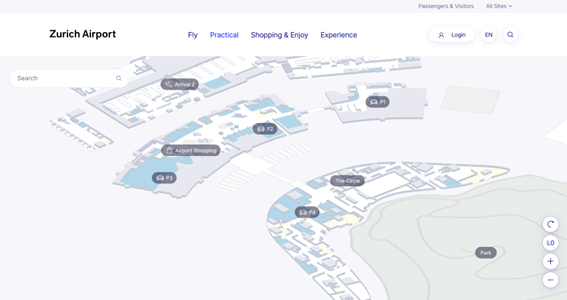
\includegraphics[scale=0.7]{planZurichAirport.png}
    \caption{Plan de l'aéroport de Zürich}
\end{figure}

\textbf{Fonctionnalités}

L'aéroport de Zurich \cite{zurich-aeroport} offre un plan non géoréférencé en 3d isométrique.
Les différents points d'intérêts affichés varient en fonction du zoom.
L'application offre un outil de recherche avec des suggestions par thème.
On peut aussi changer le fond du plan en fonction de l'étage.

Le plan ne sert que pour l'orientation des voyageurs et est donc pauvre en fonctionnalité annexe.

\textbf{Technologies utilisées}
Le site utilise le Framework réactif React js, ainsi que le module bundler webpack.  Les plans sont des images bitmap (pixellisé).

\subsection{Conclusion de l'analyse des systèmes existants}
On peut distinguer deux types d'application :
des plans interactifs qui aides des utilisateurs à s'orienter et les Géoportails qui fournissent des informations géographiques et permet de construire de nouvelles informations à l'aide d'outils de dessin vectoriel.

Cette distinction a été faite par l'EPFL, qui sépare sur deux sous-domaines différents, les deux types d'application.

Les technologies utilisées sont aussi différentes : les sites les plus complets utilisent souvent geomapfish alors que les sites les plus simples utilisent plutôt l'api google maps.


\subsection{Technologies pour les \gls{websig}}
Un \gls{websig} est une application web qui présente des données géographiques sur un plan.
Cette section présente plusieurs technologies qui facilite la mise en place de tels systèmes.

\subsubsection{Openlayers}
Openlayer \cite{openlayers} est une librairie JavaScript open source qui facilite la construction d'appllication \gls{websig}.
Elle permet de rajouter facilement des calques contenant des données géographiques en dessus d'un fond de carte.

\subsubsection{Leaflet}

Leaflet \cite{leaflet} est une librairie open source concurrente à openlayers.
Elle simple d'utilisation et légère.
On peut rajouter des plugins à la librairie afin d'étendre la librairie.

\subsection{Comparaison entre leaflet et openlayers}

Les deux librairies sont comparés dans le tableau \ref{compare}.

\begin{table}[h]
    \begin{center}
        \caption{Liste des Besoins \label{compare}}
        \begin{tabular}{l|c|c}
            Point de comparaison      & Leaflet        & Openlayers                     \\ \hline
            Simplicité d'utilisation  & simpe          & moyen                          \\
            Poids                     & Léger          & lourd                          \\
            Flexibilité               & peu flexible   & très flexible                  \\
            Nombre de format Supporté & un seul format & plusieurs format et protocoles \\
        \end{tabular}
    \end{center}
\end{table}

On peut déduire que Leaflet est plus adapté pour des petites application ou application mobile \gls{websig} alors que openlayers est plus adapté pour des applications plus complexes.

\subsubsection{Google maps API}
L'API de google maps \cite{google-maps} n'est pas open source et peut être payant.
Elle n'offre pas la possibilité de rajouter des calques au fond de carte, seulement des points d'intérêts.
Elle n'est donc pas adapté pour la construction d'application \gls{websig}

\subsubsection{GeoMapfish}
GeoMapFish est une technologie open source développé par camptocamp et permet de faciliter la construction de système d'information géographique pour le web (webGIS).
Il est composé de Ngeo pour le frontend \cite{ngeo} et de c2cgeoportal \cite{c2cgeoportal} pour le backend.

Ngeo est une librairie JavaScript qui facilite le développement d'application basé sur le Framework réactif Angular Js et l'api openLayers.
Elle utilise aussi webpack comme module bundler.

C2cGeoportal est la partie serveur construit à partir d'une image Docker. Il faut avoir une connaissance en Python pour l'utiliser.

Cette technologie est malheureusement obsolète car elle utilise une vieille version d'Angular qui est déconseillé pour le développement de nouveau projets.

\subsubsection{PostGreSQL et PostGis}
PostGreSQL est une base de données relationnelle open source, elle permet de stocker des données géographiques avec l'extension PostGis  \cite{postgis}.
Cette solution est utilisée par c2cgeoportal et dans de nombreux autres applications \gls{websig}

\section{Données existantes à disposition}
\subsection{Plans}
Des plans des étages des sites de Cheseaux et St-Roch non géoréférencé ont été fournis au format DGW, format propriétaire de AutoCAD, un logiciel de dessin techniques.

\subsection{Serveur LDAP}
Un serveur LDAP est un service d'annuaire numérique.
La HEIG-VD possède un tel annuaire et pourrait être utilisé pour fournir des informations sur certaines ressources.

\chapter{Conception de la solution}

\section{Exigences de la solution}
Pour la solution, il a été établi qu'il faudra mettre en place une interface interactive de visualisations des plans comprenant uniquement le bâtiment de Cheseaux.
Celui-ci devra afficher toute les salles du site avec leurs noms, un qualificatif (Secrétariat, salle de cours, etc.) et leur surface en mètres carrés.
Un outil de changement d'étage permettra de parcourir les différents étages du site.
L'interface sera disponible autant sur de grands écrans comme une télévision que sur de petits écrans comme les téléphones mobiles

Cette application sera hébergée sur une machine virtuel fournit par l'école.
Elle comportera une base de données qui s'occupera de stocker les données utilisées.
Un serveur API récupérera les données et les enverra a l'utilisateur.

Elle positionnera aussi certaines ressources comme les collaborateurs sur le site de la HEIG-VD.

Si le temps le permet, un outil de filtrage des ressources à affichés et/ou un outil de recherche sera aussi développé.

La solution a pour but de démontrer les possibilités qu'elle offrirai dans l'orientation des collaborateurs sur les différents sites de la \gls{heig-vd}.
Elle ne sera pas une solution utilisable par l'école.

\section{Solution envisagé}
Afin de répondre aux exigences, il a été défini que l'application sera un web,
car c'est le moyen le plus accessible pour fournir cette interface, autant sur grand et petit écran,
et sans obliger l'utilisateur à télécharger un logiciel au préalable.

Elle sera contenu sur une seule page web (single-page application)
et offrira les différentes fonctionnalités à travers ddifféerents menus.
L'affichage se modifiera en fonction de son utilisation.

\section{Explications de certains principes}
Cette section explique les principes du web, d'un reverse proxy, des container et de la base de données.
Elle s'adresse aux néophytes et vous pouvez ignorer les sous-section si vous avez des connaissances dans ces domaines.

\subsection{Web}
Premièrement, il ne faut pas confondre internet, le standard qui régit la communication entre les ordinateurs
et le web qui se base sur internet et est utilisé pas les navigateurs web pour afficher des applications.
Le second utilise les protocoles de communications HTTP et HTTPS afin d'envoyer et récupérer des données.

Lorsqu'un utilisateur tape une URL, comme www.google.ch, dans un navigateur web, il va demander à un serveur de lui envoyer
plusieurs fichiers dans des formats différents afin de permettre l'affichage de l'application web.

Sont envoyés au navigateur, des fichiers \gls{html} qui décrivent le contenu de l'application, des fichiers \gls{css} qui change l'aspect de ce contenu,
des fichiers \gls{js}, un langage de programmation, qui modifie le contenu selon les interactions de l'utilisateur avec l'application, et
les images à affichés.

Selon l'utilisation de l'application, celle-ci devra demander des données supplémentaires sur une ressources pour son fonctionnement.
Celles-ci sont envoyées dans des formats standardisé comme JSON ou XML.

\subsection{\Gls{rp}}
Un \gls{rp} permet d'accéder à différents serveurs en utilisant le même url.
Cette machine va trier les requêtes des utilisateurs
et envoyer celle-ci sur le serveur répondant à la requête.
Il peut aussi refuser des requêtes si aucun serveur ne peut les traiter.
Utiliser un \gls{rp} amène aussi plus de sécurité car on n'expose pas les autres serveurs à l'extérieur.

\subsection{\Gls{container}}
Un Container est une entité qui contient l'application ainsi que les autres programmes pour son fonctionnement.
Il est indépendant du système d'exploitation et permet d'installer les applications sur n'importe quelle machine en évitant les conflits provoqués par le système d'exploitation.
Pour exécuter un container il faut au préalable installer un logiciel gérant ceux-ci sur le sytème d'exploitation.

On peut aussi créer des images de container. Celles-ci sont en fait des fichiers regroupant les instructions qui permettent de construire les containers.
Elles peuvent être facilement dupliqués et partagés sur le web à travers des hébergeurs appelés des container registry.

\subsection{Base de données}
Une base de données est un programme qui va organiser le stockage de données sur une machine.
Elle va simplifier, l'obtention des données, l'ajout de nouvelles données, la modification et/ou la suppression de données existantes.

\section{Infrastructure}

\subsection{architecture prévu}

L'infrastructure (voir figure \ref{infra.drawio}) tourne sur une machine virtuelle de la \gls{heig-vd} et est composé de quatres containers :

\fig[width=12cm]{Architecture de l'infrastructure}{infra.drawio.pdf}

\begin{itemize}
    \item Le reverse-proxy qui renvoie les requêtes vers le serveur ou le serveur-api.
    \item Le serveur qui envoie les fichiers \gls{html}, \gls{css}, et \gls{js} au client.
    \item Le serveur api qui récolte les données dynamique depuis la base de données et les renvoie au client.
    \item La base de données qui stockent les données.
\end{itemize}

Lorsqu'un utilisateur va demander l'accès à l'application en utilisant l'url "https://tb22-bourcoud.einet.ch/", il va accéder au reverse-proxy.
Celui-ci va renvoyer la requête vers le serveur.
Ce dernier sera chargé d'envoyer les fichier \gls{html}, \gls{css}, \gls{js} ainsi que les images au client en repassant par le reverse-proxy

Par la suite, l'application a besoin d'obtenir les données des plans à afficher. Il réaccède au reverse-proxy avec une adresse commençant par "https://tb22-bourcoud.einet.ch/api/",
et la requête est renvoyé au serveur-api. Ce dernier récolte les données demandées depuis la base de données et les renvois au client en repassant par le reverse-proxy.

\subsection{Architecture idéale}
L'architecture mentionné dans la sous-section précédente est valide pour ce travail de bachelor.
Cependant, si l'école voudrait mettre en place une solution plus abouti,
il faudrait séparer chaque container dans des machines virtuelles différentes
et permettre au serveur et serveur-api de se répliquer automatiquement
ou se supprimer en fonction du nombre d'accès à l'application (scalabilité horizontal Elastique).
Cela permettrait aussi de faire face au panne d'un des containers, car d'autre maintiendrait le service.

\section{Pipeline CI/CD}
Un pipeline CI/CD est une automatisations des opérations à opérer sur les applications pour qu'elles soient mise à la disposition des utilisateurs.

\fig[width=12cm]{Pipeline CI/CD}{pipeline.drawio.pdf}

Le pipeline mis en place (voir figure \ref{pipeline.drawio}) va créer les images des containers du serveur et du serveur-api.
Les deux autres containers, vu à la section précédente, sont créé à partir d'image déjà disponibles.

Il va d'abord tester les deux applications pour éviter que des problèmes surviennent.
Ensuite il va construire les images et les publier sur un registry.

\section{Technologies utilisées}

\subsection{\gls{node} et \gls{npm}}
\gls{node} est un programme qui permet d'utiliser le Language de programmation \gls{js} en dehors des navigateurs web.

Celui-ci est très utilisé chez les développeurs et possède de nombresuses documentation. 

\gls{npm} est un programme qui gère les différentes librairies de \gls{node}.
Il permet d'ajouter, mettre à jour, supprimer des librairies utiles pour la création des applications.
Il comprend de très nombreuses librairies.

\subsection{\gls{ts}}
\gls{ts} est un Language de programmation reprenant comme base \gls{js} et lui ajoutant de nouvelles fonctionnalités utiles pour le développement.
Il se transforme (transpile) par la suite en \gls{js} lors de la construction de l'application web.

\subsection{\gls{vue3} composition}
\gls{vue3} est un Framework \gls{js} permettant de simplifier l'écriture des interractions avec le contenu de l'application web.
Elle est aussi chargé de créer du code \gls{html} et \gls{css} succeptible d'être facilement modifié.
Il offre deux styles d'écriture de code: composition ou option.
Ce projet a été écris en utilisant le style composition.

La librairie utilise une abstraction appelé component afin de créer les différents éléments de l'interface de l'application.

C'est un des Framework les plus utilisé dans le développement d'applications web.
Il a l'avantage d'être plus complète et compréhensible que React. Il est aussi moins verbeux que Angular.

\subsection{\gls{pinia}}
\gls{pinia} est une librairie associé à Vue 3 permettant de simplifier la communication de données entre les différents component.
Elle est conseillé par les développeurs de la librairie \gls{vue3} pour cette tâche.

\subsection{\gls{ol}}
\gls{ol} est une librairie JavaScript permettant d'implémenter des \gls{websig}.
Elle est très bien documenté et simplifie de nombreuses choses.

\subsection{\gls{vite}}
\gls{vite} est un environnement de développement qui permet de simuler un server pour le développement en local,
et de construire (compiler) l'application tout en optimisant la place en mémoire qu'elle prendra.

Cet environnemt est très vite installé et simplifie la compilation du programme.
Il permet aussi de créer un projet avec vue 3 déjà intégré.

\subsection{\gls{vitest}}
\gls{vitest} est la librairie de test unitaire, conseillé par l'équipe de \gls{vue3} (permet de tester des parties du code indépendamment du reste du code).
Elle est optimisé pour fonctionner avec \gls{vite} mais peut être utilisé dans d'autre projet.

\subsection{\gls{vuetest}}
\gls{vuetest} est la librairie de tests officiel de \gls{vue3} pour les components.

\subsection{\gls{nginx}}
\gls{nginx} est le serveur qui hébergera les fichiers HTML, CSS et JavaScript de l'application.

\subsection{\gls{express}}
\gls{express} est une librairie simplifiant la mise en place d'un serveur sur Node.
Il est utilisé pour créer le serveur-api.

\subsection{\gls{traefik}}
\gls{traefik} est le programme servant de \gls{rp} pour mon infrastructure.
Il est plus simple à mettre en place par rapport à ses concurrents.

\subsection{\gls{postgres} et PostGis}
\gls{postgres} est la base de données utilisé pour le projet.
Elle est open source et peut être étendu par \gls{postgis} qui elle rajoute la possibilité de stocker des données géographiques.

\subsection{\gls{docker}}
\gls{docker} est le logiciel qui gérera les container sur la machine virtuelle.


\subsection{\gls{git} et \gls{gitlab}}
\gls{git} est un programme permettant de facilement créer des versions du code source, revenir à une version précédente si besoin, et héberger son code sur des sites dédiés.

\gls{gitlab} est un hérbergeur de code source utilisant l'utilitaire \gls{git}.
Il permet aussi la collaboration entre plusieurs développeur sur une même application.

\subsection{\gls{cicd}}
\gls{cicd} est la fonctionnalité de l'hébergeur \gls{gitlab}
qui permet de lancer un pipeline CI/CD qui construira mes deux images de container.

\subsection{\gls{registry}}
\gls{registry} est l'hébergeur des deux images de container


\section{Conception de la base de données}

\subsection{explication base de données relationnelle}
Une base de données relationnelle est un type de base de données.
Au lieu de regrouper les données en une seule table,
elle permet d'en créer plusieurs et de créer des liens entre elles.
Cela permet d'éviter de la duplication de données.

Par exemple, si on veut stocker tous les numéros de salle d'un bâtiment, tous en précisant a quel étage la salle appartient,
si on utilise une seule table la mention du nom de l'étage apparaitra sur plusieurs lignes.
Par contre si on utilise une base de données relationnelle, on peut créer une table pour les salles,
une table pour les étages et créer un lien entre les deux.

Cela permet aussi d'éviter des erreurs lors d'insertion de données.

\subsection{Schéma et choix}

\fig[width=8cm]{Schéma conceptuel de la base de données}{DB_model.drawio.pdf}

La conception de la base de données est représenté dans la figure \ref{DB_model.drawio}.
Ce schéma a été conçu en notation \gls{uml}. On y aperçoit les cinq tables qui seront décris après.
Si on étudie bien chaque table, on peut remarquer que certains champs aurait pu être séparé dans d'autres tables afin d'éviter des duplications. 
Par exemple, le champ type dans room.

Il a été choisi de laisser ces duplications
car cela permet de simplifier le transfert de données géographiques sous format geoJson
(standard de fichier JSON pour le stocker des données géographiques).

\subsection{Tables et  relations}
\subsubsection{Building}
La table Building représente un bâtiment et est composé des champs suivants :

\begin{itemize}
    \item id : l'identifiant unique du bâtiment
    \item name : le nom du bâtiment
    \item x : la coordonnées x pour centrer le bâtiment sur une projection ESPG : 3857.
    \item y : la coordonnées y pour centrer le bâtiment sur une projection ESPG : 3857.
    \item ground\_floor : le nom de l'étage du rez-de-chaussée
    \item rotation : la rotation par rapport au nord pour une meilleure visualisation du bâtiment.
    \item zoom : le zoom pour \gls{ol} pour une meilleure visualisation du bâtiment.
    \item min\_zoom : le zoom minimum pour \gls{ol} que pourra utiliser l'utilisateurs.
    \item max\_zoom : le zoom maximum pour \gls{ol} que pourra utiliser l'utilisateurs.
\end{itemize}

La table possède les relations suivantes :
\begin{itemize}
    \item Floor : le bâtiment possède plusieurs étage.
    \item Resource : le bâtiment peut posséder plusieurs ressources
\end{itemize}

\subsubsection{Floor}
La table floor représente un étage d'un bâtiment et est composé des champs suivants :

\begin{itemize}
    \item id : l'identifiant unique de l'étage.
    \item name : le nom de l'étage.
\end{itemize}

La table possède les relations suivantes :
\begin{itemize}
    \item Building : l'étage appartient à un bâtiment.
    \item Resource : l'étage peut posséder plusieurs ressources.
    \item Floor\_geometry : l'étage est composé de plusieurs données géométriques
\end{itemize}

\subsubsection{Floor\_geometry}
La table Floor\_geometry représente des données géométriques associé à un étage et est composé des champs suivants :

\begin{itemize}
    \item id : l'identifiant unique de la donnée géométriques.
    \item type : le type de géométrie.
    \item geomtry : la donnée géométrique.
\end{itemize}

La table possède la relations suivante :
\begin{itemize}
    \item Floor : les données géométriques appartiennent à un étage.
\end{itemize}

\subsubsection{Room}
La table Room représente une salle d'un bâtiment et est composé des champs suivants :

\begin{itemize}
    \item id : l'identifiant unique de la salle.
    \item name : le nom de la salle. (ex: E01)
    \item second\_name : le second nom de la salle s'il y en a un (ex: marketing). Peut ne pas être renseigné.
    \item type : le type de salles. (ex: salle de cours) Peut ne pas être renseigné.
    \item area : la surface de la salle. Peut ne pas être renseigné.
    \item capacity : le nombre de place d'une salle. Peut ne pas être renseigné.
    \item geometry : les données géographiques de la salle.
\end{itemize}

La table possède les relations suivantes :
\begin{itemize}
    \item Floor : la salle appartient à un étage.
    \item Resource : la salle peut posséder plusieurs ressources
\end{itemize}

\subsubsection{Resource}
La table Resource représente tout type de ressources comme les extincteurs, les toilettes ou les ascenseurs
que l'on peut trouver dans d'un bâtiment, un étage, une salle et est composé des champs suivants :

\begin{itemize}
    \item id : l'identifiant unique de la ressource.
    \item name : le nom de la ressource.
    \item type : le type de la ressource.
    \item image\_name : le nom de l'image associé à la ressource.
    \item description : la description de la ressource.
    \item localisation : la localisation de la ressource dans une projection ESPG : 3857.
\end{itemize}

La table possède les relations suivantes :
\begin{itemize}
    \item Building : la ressource est associé à un bâtiment.
    \item Floor : la ressource peut être associé à un étage.
    \item Room : la ressource peut être associé à une salle.
\end{itemize}

\section{Planification de la mise en place de la solution}
Ce chapitre présente la plannification du projet et les principales étapes.

\begin{figure}[H]
    \caption{Planning du projet (version agrandi en annexe)}
    \centering
    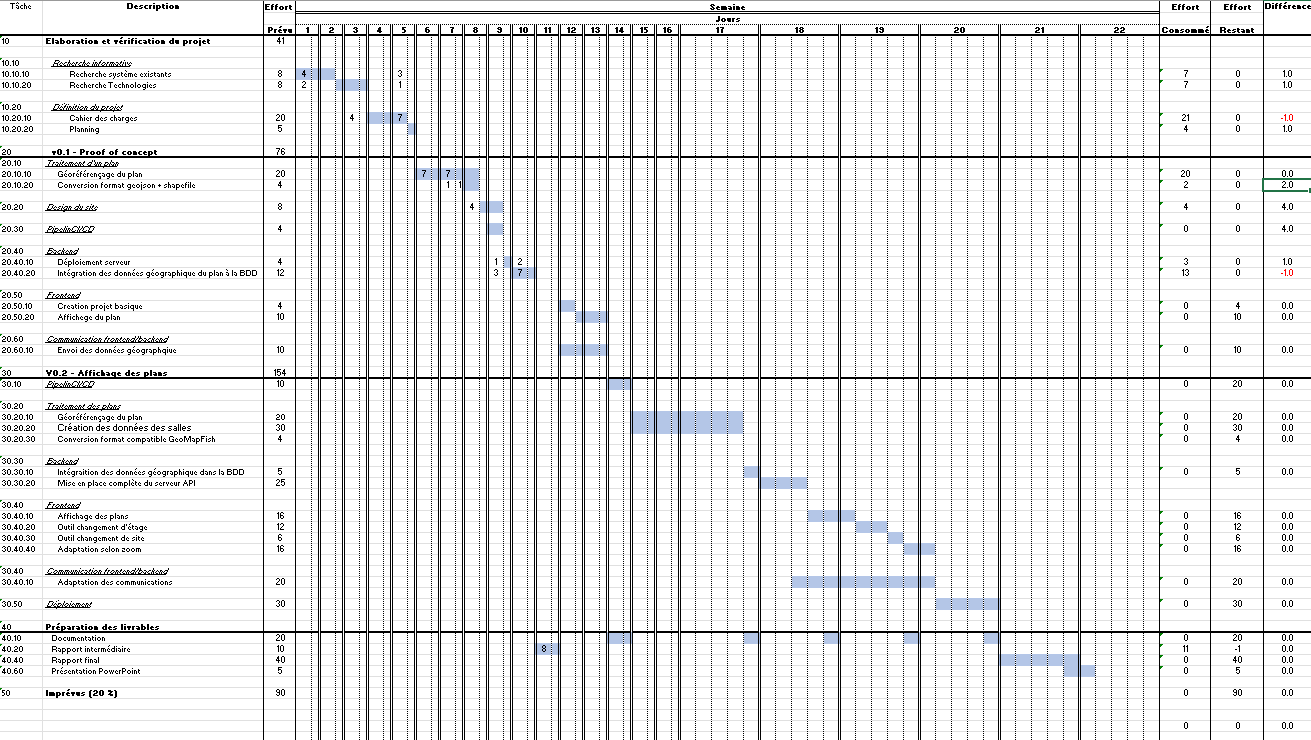
\includegraphics[scale=0.5]{planning.png}
\end{figure}

\subsection{Echéances et étapes}
Les principales échéances de ce travail sont le rendu d'un cahier des charges le jeudi 14 avril 2022,
le rendu d'un rapport intermédiaire le lundi 16 mai 2022,
le rendu final du projet le vendredi 29 juillet 2022 et
finalement une défense qui aura lieu entre le 22 août et le 16 septembre.

Il y'a deux grandes étapes de prévus :
une première version servant de proof of concept qui se finira le dimanche 29 mai 2022
et une deuxième version qui sera la version final du projet pour le 29 juillet 2022.
Ces versions sont décrites dans les sous-sections suivantes.

D'autres versions pourront être mis en place par la suite afin de rajouter des fonctionnalités,
mais cela demanderait plus de temps que ce qui a été planifié pour le TB.

\subsection{Elaboration du projet}
La première étape était d'analyser les informations sur les projets websig. Pour cela 16 heures ont été planifé.
Puis, il fallait préciser le travail à éxécuter en rédigeant un cahier des charges et un planning. Pour cela 25 heures ont été planifié.

\subsection{Première version du projet}
La première étape, était la prise en main des différentes technologies afin de vérifier la faisabilité du projet.
Le but était de mettre en place une application websig minimaliste, n'affichant qu'un étage avec ses salles et n'offrant pas de fonctionnalités supplémentaires.

Pour réaliser cette version il a été établi qu'il faudrait

\begin{itemize}
    \item Traiter un des plans et créer les données géographiques, 24 heures.
    \item Concevoir le design de l'application, 8 heures.
    \item Mettre en place un pipeline CI/CD, 4 heures.
    \item Création du serveur-api et de la base de données, 16 heures.
    \item Création du frontend, 24 heures.
\end{itemize}

\subsection{Deuxième version du projet}
Le deuxième étape, après avoir vérifié la faisabilité du projet, était la mise en place de la solution finale.


Pour réaliser cette version il a été établi qu'il faudrait

\begin{itemize}
    \item Traiter les plans du site de Cheseaux et créer les données géographiques, 54 heures.
    \item Mettre en place le serveur-api et de la base de données, 30 heures.
    \item Mettre en place le frontend, 70 heures.
    \item Déploiement de l'application sur la machine virtuelle, 30 heures.
\end{itemize}

\subsection{Documentation du travail}
La documentation du travail étant importante, il a aussi fallu planifié celle-ci:

\begin{itemize}
    \item Documentation du code, 20 heures.
    \item Rapport intermédiaire, 10 heures.
    \item Rapport final, 40 heures.
    \item Présentation, 5 heures.
\end{itemize}

\subsection{Aperçu global}

\begin{figure}[h]
    \centering
    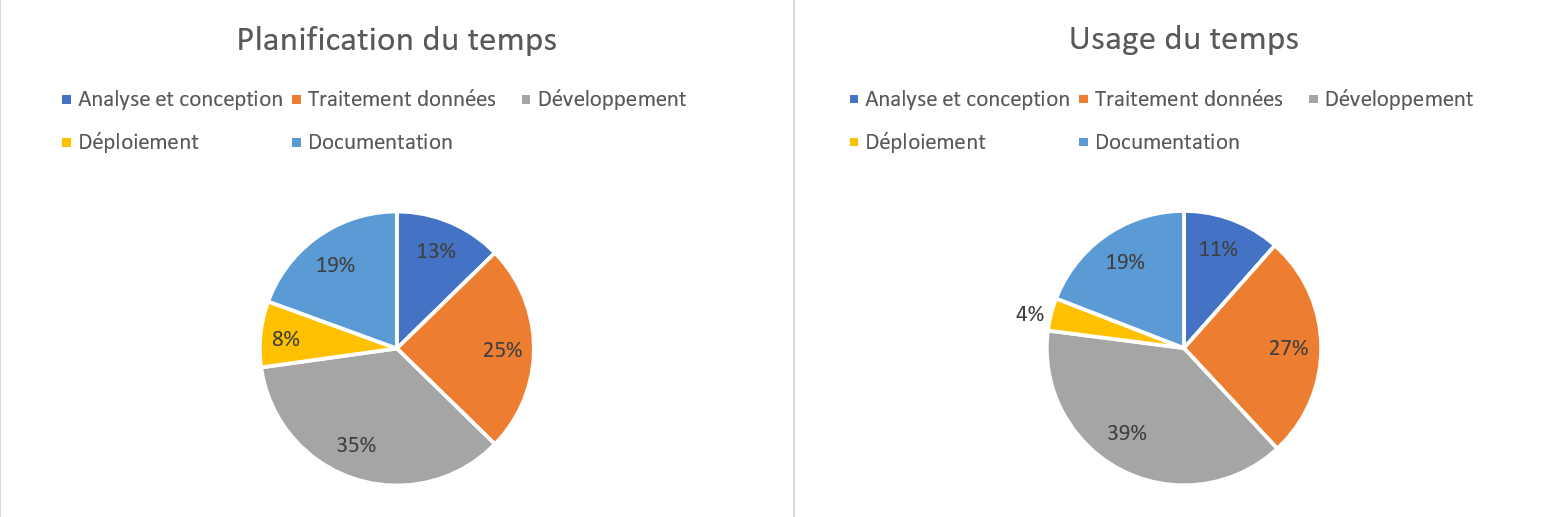
\includegraphics[scale=0.4]{RepartitionTemps.png}
    \caption{Repartition du temps}
    \label{fig:temps1}
\end{figure}

La figure \ref{fig:temps1} résume le temps alloué aux différentes catégories de travail.


\section{Design de la solution}

Cette section décrit les designs imaginé pour la solution.
Ceux-ci ne sont pas précis et seront susceptible de changer lors de l'implémentation.
De plus, des outils comme le menu de filtrage ou la recherche risque de ne pas être implémenté.

\subsection{Design global}

\begin{figure}[h]
    \centering
    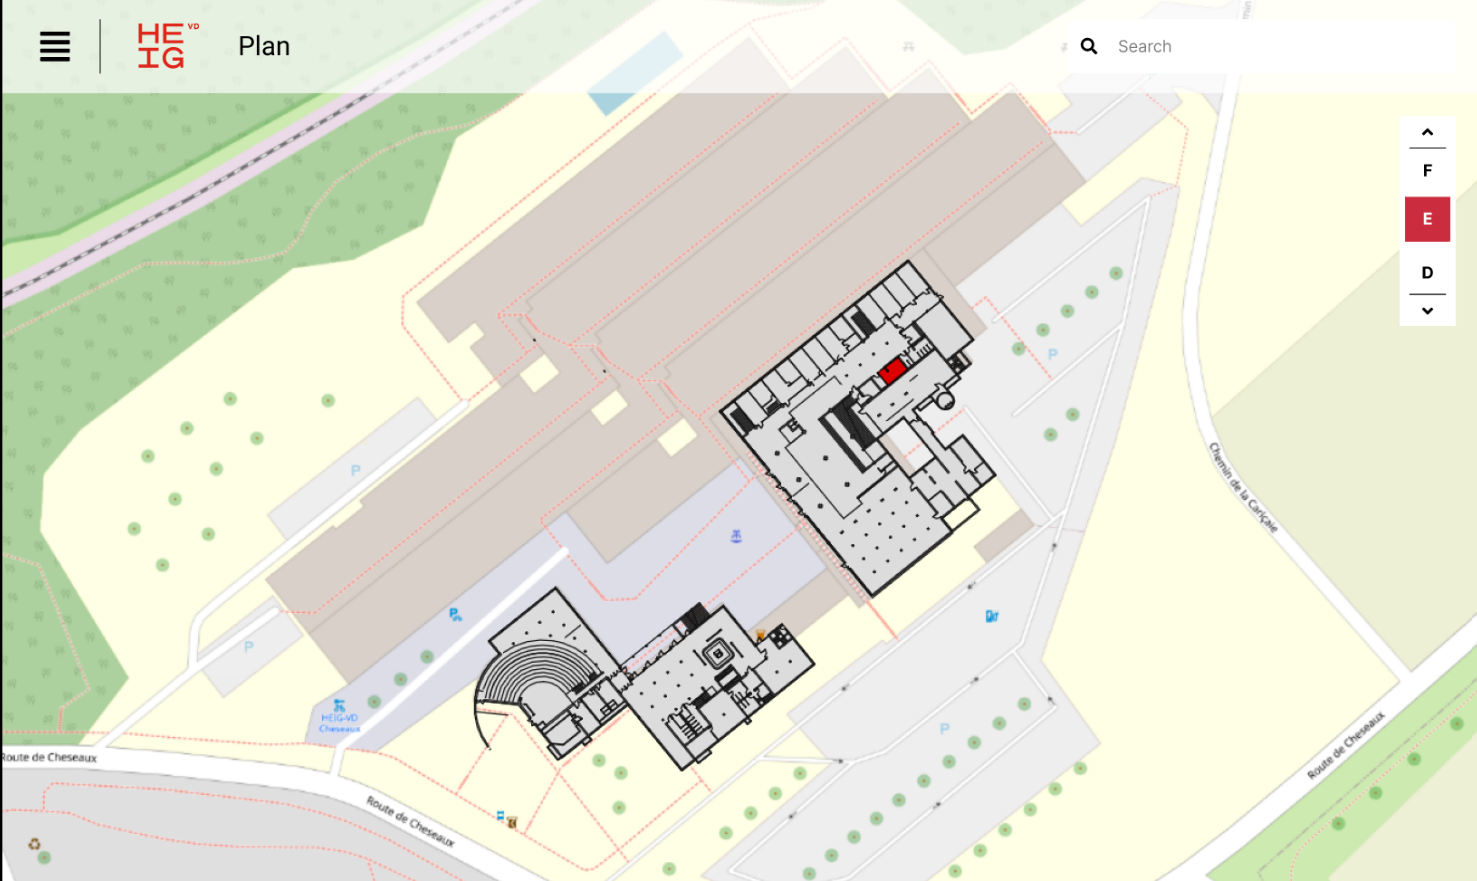
\includegraphics[scale=0.4]{designGlobal.png}
    \caption{Design global}
    \label{fig:globalDesign}
\end{figure}

Le design global (voir figure \ref{fig:globalDesign}) essaie de respecter la charte graphique du site heig-vd.ch/ en utilisant son logo, son code couleur et la transparence du header.
Le design a été conçu pour un écran au format 16/9, mais l'application sera aussi disponible pour d'autre types d'écrans.
L'application sera sur une seule page sans scroll principal
(Des scrolls secondaire seront possibles pour des fonctionnalités comme la fenêtre d'informations).

Sur cette page on peut accéder à plusieurs outils :

\begin{itemize}
    \item Un menu pour filtrer les informations à afficher en cliquant sur le bouton en haut à gauche.
    \item Un outil de recherche à droite du header
    \item Un outil de changement d'étage à droite de la fenêtre
    \item Une fenêtre d'information en cliquant sur une salle ou en ayant effectué une recherche
\end{itemize}

\subsection{Outil de changement d'étage}

\begin{figure}[h]
    \centering
    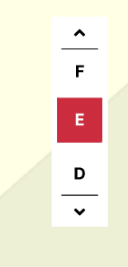
\includegraphics[scale=1]{designChangementEtage.png}
    \caption{Design de l'outil de changement d'étage}
    \label{fig:floorChange}
\end{figure}

L'outil de changement d'étage (voir figure \ref{fig:floorChange}) permet de modifier l'étage affiché sur le plan.
Il indique, érit en blanc sur fond rouge, l'étage actuel auquel se trouve l'utilisateur.
On pourra modifier celui-ci en cliquant sur les flèches.
L'outil indique aussi l'étage précédent et suivant
afin d'éviter que l'utilisateur ne sache pas sur quelle flèche cliquer pour accéder à l'étage désiré.

\subsection{Fenêtre d'informations}

\begin{figure}[h]
    \centering
    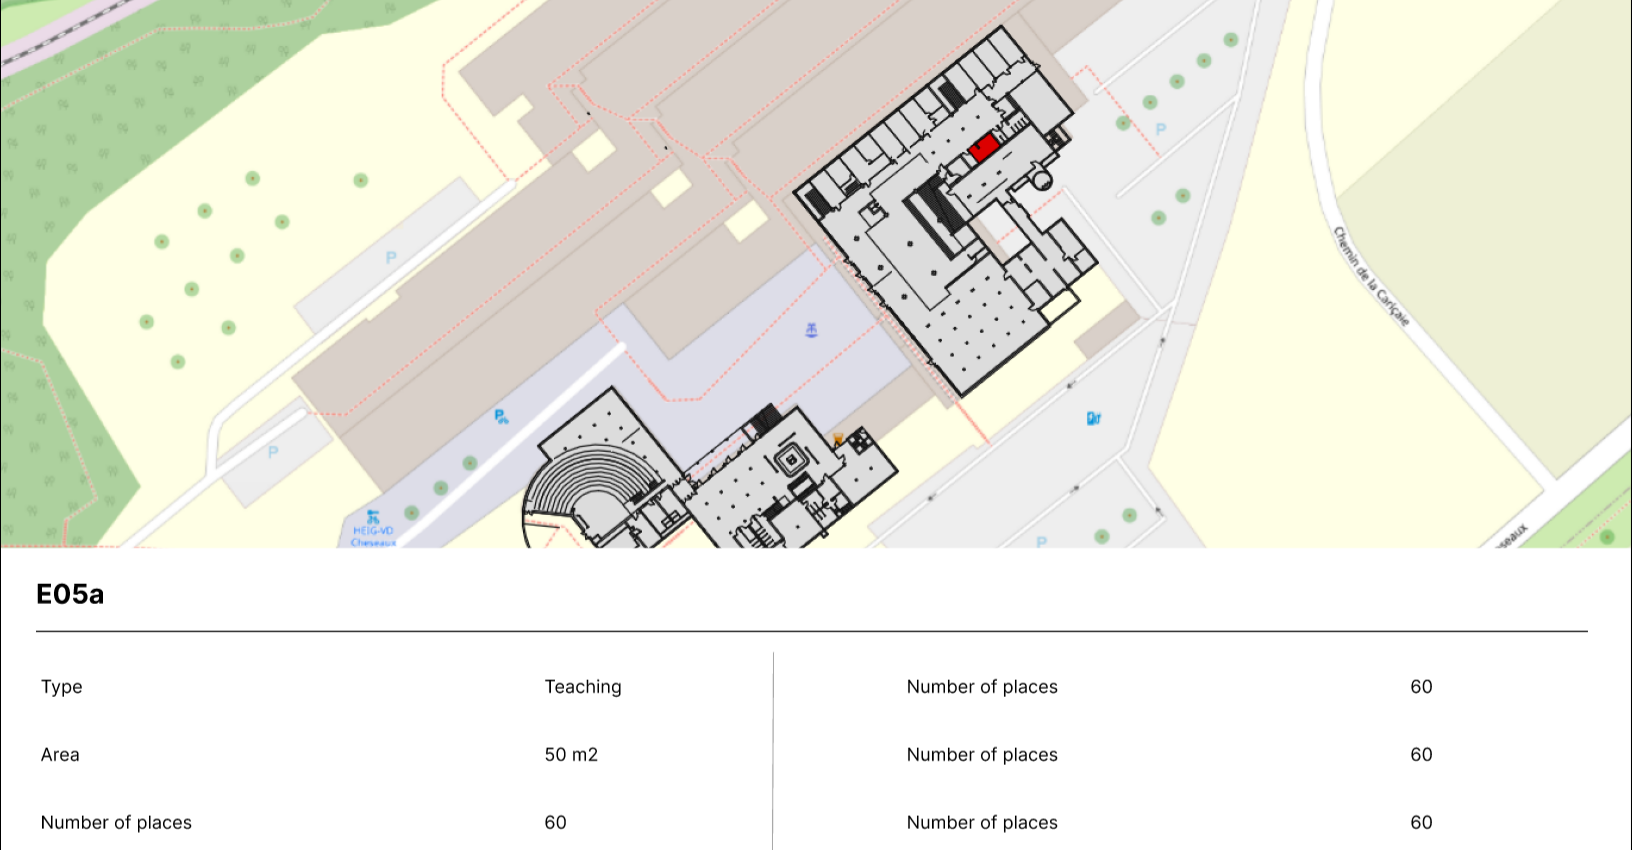
\includegraphics[scale=0.4]{designInfo.png}
    \caption{Design de la fenêtre d'information}
    \label{fig:infoPanel}
\end{figure}

La fenêtre d'informations (voir figure \ref{fig:infoPanel}) s'affichera sur le bas, lors d'un clic sur une salle ou après avoir exécuté une recherche.
Elle présentera les informations concernant la salle.
Pour la fermer, l'utilisateur pourra cliquer en dehors de la fenêtre.

\subsection{Menu de filtrage}

\begin{figure}[h]
    \centering
    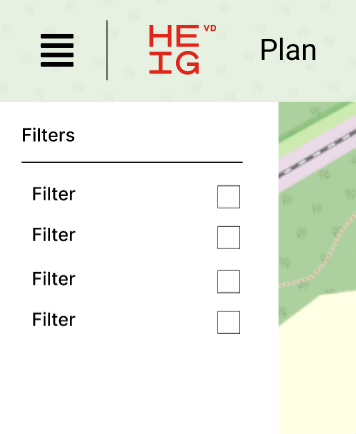
\includegraphics[scale=0.5]{designFilter.png}
    \caption{Design du menu de filtrage}
    \label{fig:filterPanel}
\end{figure}

Le menu de filtrage (voir figure \ref{fig:filterPanel}) s'affichera sur la gauche de l'écran, lorsque l'utilisateur cliquera sur le bouton en haut à droite.
Elle permettra d'ajouter ou enlever des éléments à afficher sur la carte.
Pour sortir du menu, l'utilisateur pourra cliquer en dehors de celui-ci, ou à nouveau sur le bouton.

\subsection{Outil de recherche}

\begin{figure}[h]
    \centering
    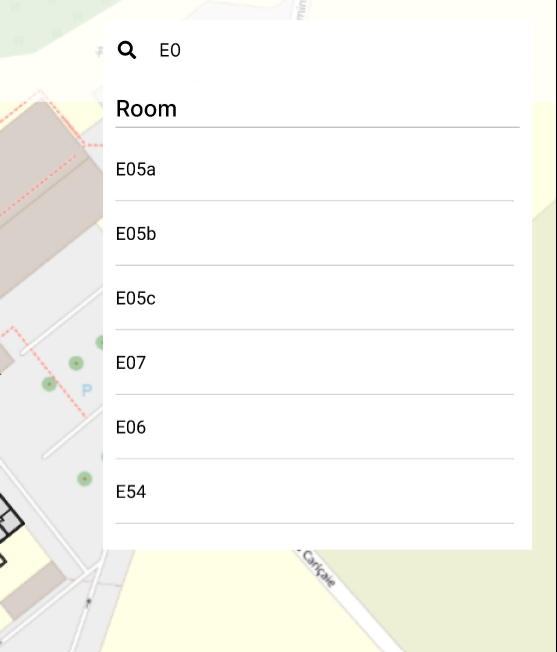
\includegraphics[scale=0.3]{designRecherche.png}
    \caption{Design de l'outil de recherche}
\end{figure}

Lorsque l'utilisateur commencera à taper des caractères dans le formulaire de recherche celui ci proposera un menu de suggestions.
Si l'utilisateur clique sut la touche entrée ou sur une des suggestions, l'affichage du plan se modifiera pour afficher la ressource demandé.


\chapter{Réalisation de la solution}

\section{Création des données géographiques}

La plupart des données géographiques devait soit être traitées, soit être créées.
Cette section explique le processus de travail afin d'obtenir ces données et comment elles ont étés stockés dans la base de données.

La solution proposé dans cette section est critiqué dans le chapitre de Conclusion.

\subsection{\gls{qgis}}
\gls{qgis} est un logiciel de système d'information géographique, qui permet de visualiser, traiter et diffuser ces informations.
Il a été utilisé dans ce projet afin de traiter les plans, et créer les autres données géographiques.

Un apprentissage du logiciel a été nécéssaire afin de mettre en oeuvre une solution pour le projet.

\subsection{Les plans}
Les plans mis à disposition sont stockés dans des fichiers DWG, un format propriétaire du logiciel de dessin technique AutoCAD, utilisé pour créer les plans d'architecte.
Ce format représente les informations géographiques sous format vectoriel, représentation d'une image non pixellisé qui ne dépend pas de la résolution.
Les données sont séparés sur plusieurs calques.

Les plans ne sont pas encore géoréférencé, c'est à dire qu'il se trouve dans un système local de coordonnées
et qu'il faut les traiter pour les placer au bon endroit sur un autre système de coordonnées.

\subsection{Géoréférencement des plans dans \gls{qgis}}
\begin{figure}[h]
    \centering
    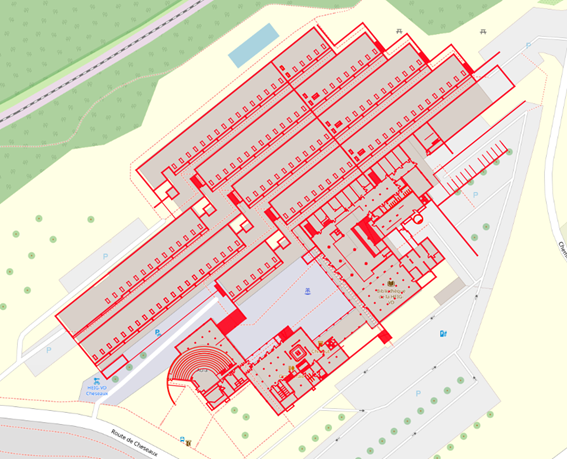
\includegraphics[scale=0.5]{Géoréférencement.png}
    \caption{Résultat final du géoréférencement d'un plan}
    \label{fig:georeferencement}
\end{figure}

Avant même d'ouvrir le logiciel \gls{qgis}, il faut choisir la projection (système de coordonnées) dans laquelle les plans seront géoréférencé.
Pour ce projet, la norme ESPG : 3857 - WGS 84 / Pseudo-Mercator, car c'est celle utilisé par open street map.

Dans une première étape, il a fallu sélectionné les calques contenant les informations utiles pour le projet,
puis importer ceux-ci grâce à l'outil intégré dans QGIS "Import Layers from DWG/DXF "

La deuxième étape était le géoréférencement.
Pour ce faire, le fond de carte Open Street Map a été intégré et servira de référence pour le placement des calques.
Le plugin " Vector Bender " a été utilisé pour effectué une transformation affine sur les plans, afin de les déplacer vers la bonne référence.
Finalement les nouvelles données ont été enregistré dans le format " ESRI shapefile " qui est plus adapté pour les manipulations dans ce logiciel.

Le résultat final peut être observé avec la figure \ref{fig:georeferencement}

\subsection{Création des informations géographiques}

\begin{figure}[h]
    \centering
    \includegraphics[scale=0.6]{créatioNgeodata.png}
    \caption{Résultat final de la création d'informations de l'étage E}
    \label{fig:polygones}
\end{figure}

Une fois le géoréférencement fini, seul le tracé de chaque étage était visible.
Il a fallu créer les données suivantes :

\begin{itemize}
    \item Le contour des étages sous forme de polygones au lieu de lignes
    \item Le contour des salles sous forme de polygones
    \item La localisation des ressources sous forme de points
\end{itemize}

La figure \ref{fig:polygones}, montre la création du contour de l'étage E et des ses salles.
La figure \ref{fig:ressources}, montre la création des localisation des ressources.

Le travail de création des données géographiques pour le site de Cheseaux a pris beaucoup de temps.

Lors de la création de ces données, il y a la possibilité de rajouter des métadonnées à chaque informations géographiques
(données suppllémentaires). Cependant ce travail n'as été fait que pour la localisation des ressources par méconnaissance de cette possibilité.
Le faire pour les autres, aurait pris du temps pour un travail qui a déjà été fait.


\begin{figure}[h]
    \centering
    \includegraphics[scale=0.6]{data-créationRessources.png}
    \caption{Résultat final de la création d'informations des ressources}
    \label{fig:ressources}
\end{figure}

\subsection{Problèmes rencontrés avec \gls{qgis}}
Le premier problème rencontré lors de l'utilisation du logiciel était les recherches de solutions pour le géoréférencement,
Certains outils ne faisait pas de transformation affine correcte ou émettait des erreurs.

Un second a été que Le plugin "Vector Bender" nécessite que tous les calques utilisés pour la transformation affine utilise la même projection.

\subsection{Exportation et arborescence de fichiers}
Afin de pouvoir traiter les données et les placer dans la base de données,
il fallait exporter celle-ci depuis le logiciel dans un format facilement lisible par un programme informatique.
Le choix a été fait sur le format \gls{geojson}.

Ceux-ci ont été exporté dans l'arborescence de fichier suivante :
Le dossier racine contient des dossiers portant le nom des différents bâtiments.
Ceux-ci contiennent des dossiers portant le nom de chaque étage ainsi qu'un dossier contenant les fichiers \gls{geojson} des ressources lié au bâtiment.
Les dossiers des étages contiennent les fichiers \gls{geojson} des informations géographiques relatif à l'étage, ainsi qu'un dossier portant le nom rooms.
Ce dernier contient les fichiers \gls{geojson} relatifs à chaque salle.

Cette arborescence sera utile pour la création des scripts SQL.

\subsection{Création des script SQL}
SQL est un language pour gérer une base de données relationnelle comme PostGreSQL.
Celui permet de créer la base de données et les tables, récupérer les données, d'en insérer de nouvelles, d'en modier ou d'en supprimer.

Pour ce projet, un programme  a été créé afin de lire les fichiers dans l'arborescence décris dans la sous-section précédente
et créer trois fichiers SQL. Un pour la création de la base de données, un pour la création des tables et un pour l'insertion des données géographique dans la base de données.

Ils seront utilisé pour mettre en place la base de données lors du déploiement de l'application.

\section{Backend | Serveur-api}
Le serveur API s'occupe de récupérer les données depuis la base de données, et de les envoyer à l'application web.

\subsection{Organisation du code source}

\begin{figure}[h]
    \centering
    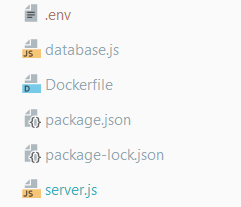
\includegraphics[scale=0.9]{backend_source_code.png}
    \caption{arborescence de fichier du server-api}
    \label{fig:backend_source_files}
\end{figure}

La figure \ref{fig:backend_source_files} contient deux fichiers importants: server.js qui implémente le serveur express et les différentes routes,
et database.js qui contient le code de connection à la base de données et les requêtes SQL pour acheminer les données.

\subsection{Communications}

\fig[width=8cm]{Diagramme de séquence représentant les communications pour le serveur api}{serverApi_sequenceDiagram.drawio.pdf}

Le diagramme de la figure \ref{serverApi_sequenceDiagram.drawio.pdf} présente les communications entre le client web,
le serveur-api, et la base de données. Le client web va d'abord faire une requête HTTP au serveur-api.
Ce dernier va exécuter une requête SQL à la base de données afin de récupérer les données.

Lorsque qu'il reçoit une réponse, il va vérifier si les données sont existentes.
Si elles le sont, il va les traiter puis les envoyer sous format JSON au client web, avec le code de status, propre au protocole HTTP, 200 OK.
Dans le cas contraire, il va envoyer un message d'erreur avec le code de statut 400 Bad request.

\subsection{Routing}

L'application web, a besoin d'acheminer différentes ressources. Pour ce faire, elle accède au serveur-api en utilisant différentes urls liées aux données désirés.
Ces urls sont appelés des routes.

Les routes seront présentés avec la deuxième partie de l'url.
par exemple le site factice www.site.web/element1/:element2 sera présenté seulement avec /element1/:element2.

De plus, si un des éléments est précédé par deux points, cela veut dire qu'il peut prendre n'importe quelle valeur.
Par exemple /element1/:element2 peut être écrit /element1/356 ou /element1/bonjour
Cette valeur sera utilisé lors de la requête SQL et récupérera des données si cela correspond à des entrées dans la base de données.

Voici la liste de chaque route et des données récupérées :

\begin{itemize}
    \item '/api/buildings' récupère les informations sur tous les bâtiments.
    \item '/api/buildings/:buildingId/floors' récupère les informations sur les étages d'un bâtiment.
    \item '/api/buildings/:buildingId/resources' récupère les informations sur les ressources liés à un bâtiment mais pas à un étage.
    \item '/api/floors/:floorId/features' récupère les informations liées à un étage.
    \item '/api/rooms/:roomId/resources' récupère les ressources liées à une salle.
    \item '/api/rooms/search/:search' récupère les noms des salles selon une recherche.
    \item '/api/rooms/:name' récupère les informations d'une salle selon son nom.
\end{itemize}

\subsection{ORM}
Ce projet n'utilise pas d'ORM,
une technique de programmation qui facilite la récupération des données prêt à l'emploi, à partir d'une base de données, pour le langage de programmation,
car :

\begin{itemize}
    \item Les données sont récupérés sous format JSON, qui est utilisable pas le Language de programmation \gls{js} sans trop de transformation.
    \item Certaines requêtes sont spécifique à l'extension \gls{postgis} et aurait demandé d'étendre les fonctionnalités de l'ORM
    \item Le serveur-api ne fait que peu de traitements des données avant de les renvoyer au client web.
\end{itemize}



\section{Frontend}

Le frontend est un projet qui sera transformé en fichiers \gls{html}, \gls{css} et \gls{js} avant d'être servi par le serveur.

\begin{figure}[h]
    \centering
    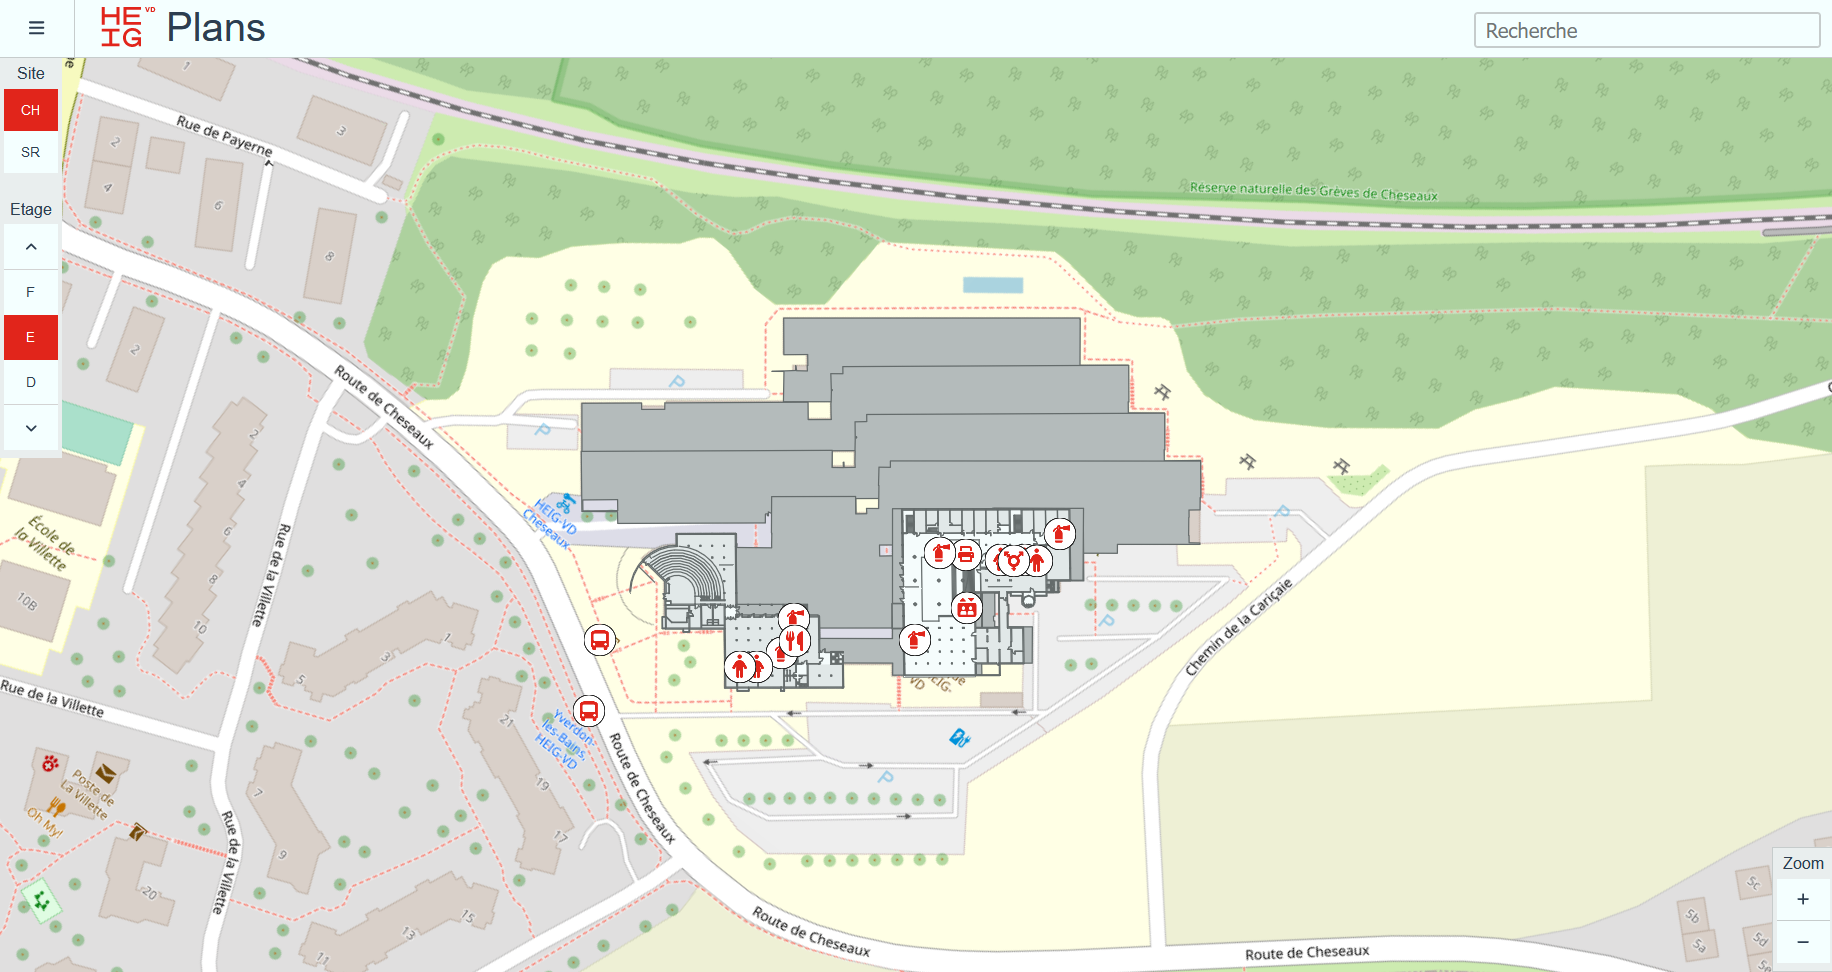
\includegraphics[scale=0.3]{frontend-global.png}
    \caption{Affichage global de l'application}
\end{figure}

\subsection{Organisation du code source}

\begin{figure}[h]
    \centering
    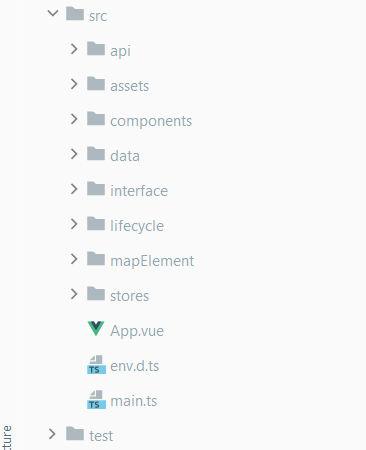
\includegraphics[scale=0.7]{frontend-source-organisation.png}
    \caption{Organisation du code source}
    \label{fig:fichier-source}
\end{figure}

Le code de l'application (voir figure \ref{fig:fichier-source}) se trouve dans le dossier src et les tests dans le dossier test.
A la racine du dossier src se trouve le fichier main.ts qui est la porte d'entrée de l'application,
ainsi que le fichier app.vue qui est le component vue principal qui englobe tous les autres components.

Le reste du dossier est composé des dossier suivant :
\begin{itemize}
    \item api : contient le code permettant de communiquer avec le serveur-api
    \item assets : contient les images de l'application
    \item component : contient les component vue. Ils sont organisé dans des sous-dossiers par type de component.
    \item interface : contient les interfaces \gls{ts} qui définissent des types d'objet
    \item lifecycle : contient le code gérant la Stratégie de récolte des données.
    \item mapElement : contient des élements concernant la librairie \gls{ol}
    \item stores : contient les fichiers permettant de communiquer des informations entre plusieurs vue component.
\end{itemize}

\subsection{Stratégie de récupération des données}

\fig[width=12cm]{Schéma de la stratégie de récupération des données}{frontend_flowChart.drawio.pdf}

La récolte des données nécéssaire pour le bon fonctionnement de l'application se fait en deux temps(voir figure \ref{frontend_flowChart.drawio.pdf})
Le choix de le faire ainsi permets à l'utilisateur d'accéder plus rapidement à l'application sans devoir attendre que celle-ci soit complétement prêtes.
Dans un premier temps l'application va récupérer les données nécéssaires via le serveur-api,
afin d'afficher le fond de carte, l'étage E de Cheseaux et les ressources associé à cet étage.
L'utilisateur pourra alors accéder au plan sans trop d'attente.

Dans un deuxième temps, il va récupérer les informations géographiques de tous les bâtiments contenu dans la base de données,
ainsi que leur étage.

Toutes les données récupérés lors de ces deux étapes sont mise en cache (stocker temporairement sur la machine de l'utilisateur),
afin d'éviter de multiplier des mêmes requêtes, et permettre une navigation fluide sur la carte sans temps de latence.

Lors de l'utilisation de l'outil de recherche, des requêtes sont encore effectués pour récupérer les données de salle.

\subsection{\gls{ol} layers}
\gls{ol} permet pour la création de \gls{websig} de séparer les données géographiques sur des calques (layers) superposés les uns sur les autres.
Afin d'afficher les plans, les données géographiques ont été séparé sur les calques suivant :

\begin{itemize}
    \item osmLayer : calque affichant le fond de carte fournis par open street map.
    \item backgroundLayer : calque affichant les contours du bâtiment.
    \item polygonLayer : calque affichant le fond de l'étage sélectionné.
    \item lineLayer : calque affichant les lignes provenant du plan de l'étage selectionné.
    \item labelsLayer : calque affichant les noms des salles.
    \item resourceLayer : calque affichant les icones des ressources.
\end{itemize}

Quand un utilisateur veut changer d'étage ou de bâtiment, les sources de données des calques sont remplacés par d'autres sources.

\subsection{Fonctionnalités}

\subsubsection{Ecran de chargement}

\begin{figure}[h]
    \centering
    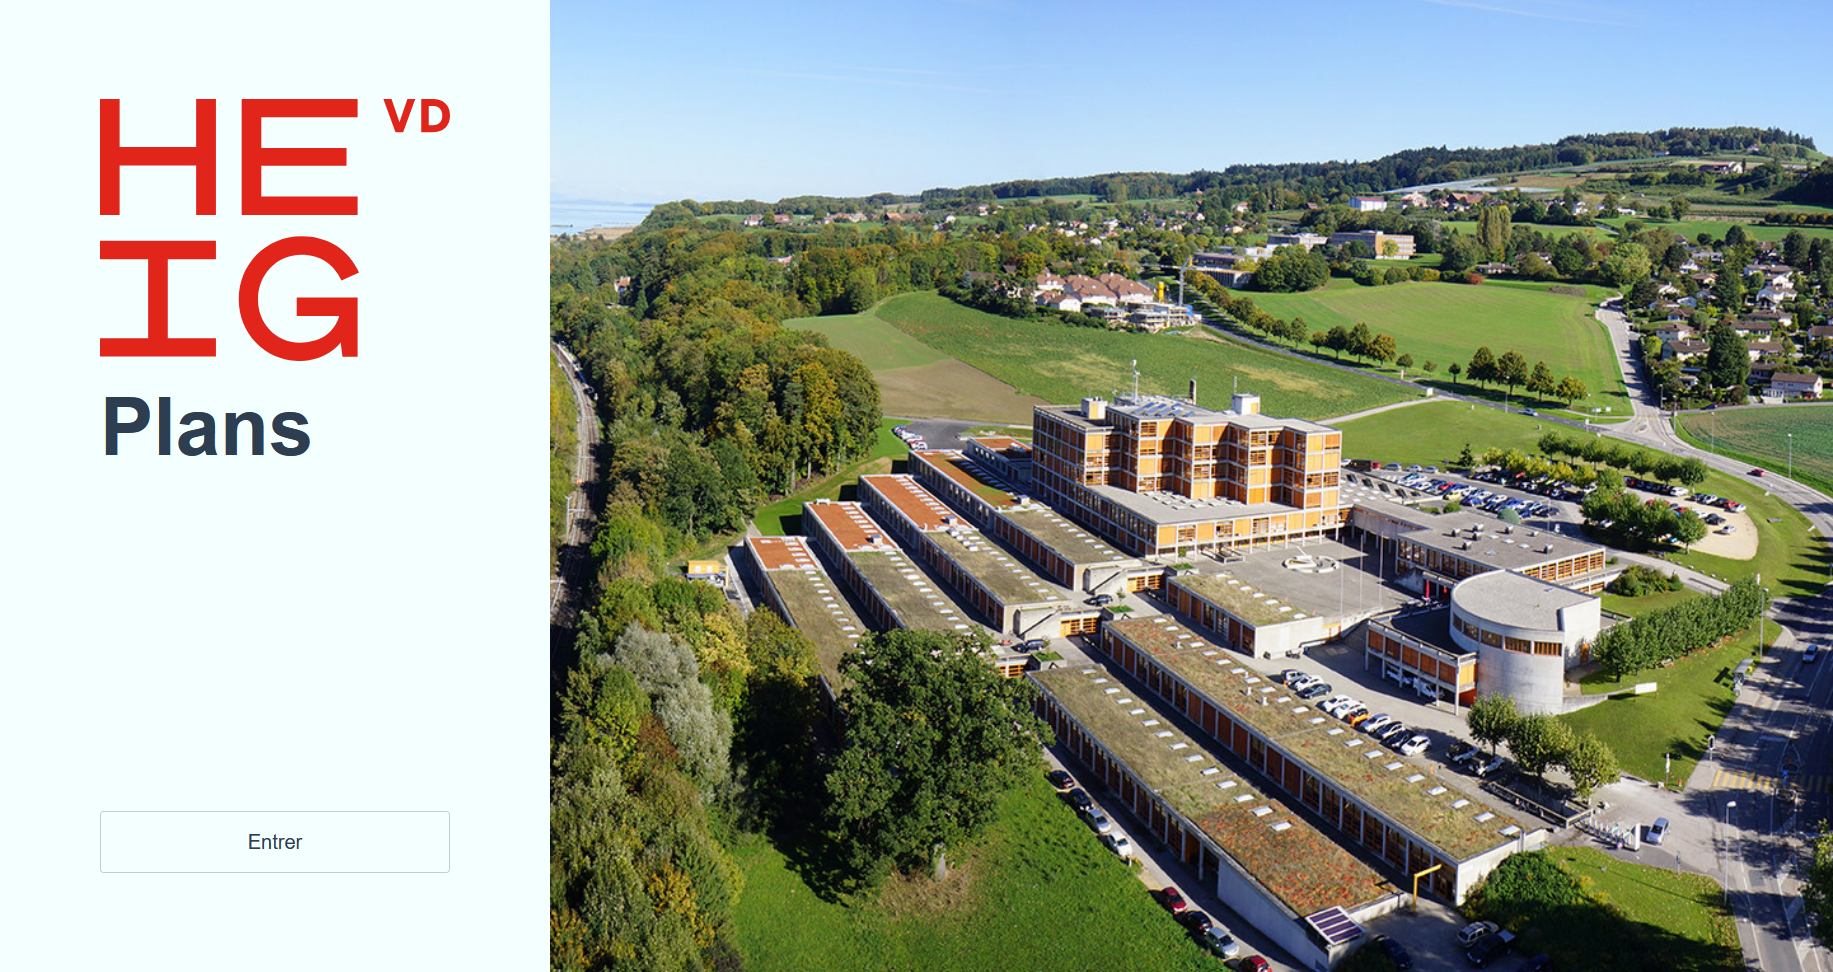
\includegraphics[scale=0.3]{frontend-loading-screen.png}
    \caption{Ecran de chargement}
    \label{fig:ecran-chargement}
\end{figure}

L'écran de chargement (voir figure \ref{fig:ecran-chargement}) permet de faire patienter l'utilisateur jusqu'au chargement des données essentielles à l'affichage du plan
(1ère étape de la récupération des données ).
Elle permet aussi de donner un aperçu du bâtiment de Cheseaux et donc offrir une meilleure compréhension du plan par la suite.

Afin d'accèder au plan l'utilisateur doit cliquer sur un bouton. Cela permet de laisser le temps de comprendre le bâtiment de Cheseaux.

\subsubsection{Outil de changement de bâtiment}

\begin{figure}[h]
    \centering
    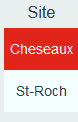
\includegraphics[scale=0.8]{frontend-buildingChange.png}
    \caption{Outil de changement de bâtiment}
    \label{fig:changement-batiment}
\end{figure}

L'outil de changement de bâtiment (voir figure \ref{fig:changement-batiment}) permet de naviguer d'un bâtiment à l'autre.
Le bâtiment actuellement selectionné est écris en blanc sur fond rouge. Les autres bâtiment sont des boutons cliquable.
Tous les textes  sont des abréviations des noms des bâtiments, et lorsque l'utilisateur passe le curseur au dessus de l'outil,
Le nom entier s'affiche à la place des abréviations.

Lors d'un clic sur un des ces boutons le plan change d'affichage et se centre sur le bâtiment nouvellement sélectionné.
Les sources des calques sont modifié en conséquence.
L'étage qui est selectionné est le rez-de-chaussée du bâtiment, mentionné dans la base de données.
L'outil de changement d'étage s'adapte aussi en changeant la liste des étages.
Cependant ceci ne se vérifie pas dans la version final car les données des étages de St-Roch ne sont pas implémenté dans la base de données
et que le comportement normal lors de données manquantes est de ne pas modifier la liste.

Lors de la conception du design cet outil n'avait pas été planifié.

\subsubsection{Outil de changement d'étages}

\begin{figure}[h]
    \centering
    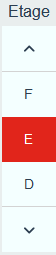
\includegraphics[scale=0.8]{frontend-floorChange.png}
    \caption{Outil de changement d'étages}
    \label{fig:changement-étage}
\end{figure}

L'outil de changement d'étage (voir figure \ref{fig:changement-étage}) permet de naviguer à travers les étages d'un bâtiment.
Il présente l'étage selectionné, ainsi que l'étage suivant et l'étage précédent.

Lors d'un clic sur la flèche du haut ou sur l'étage suivant, l'outil sélectionne l'étage suivant
et change les sources des calques. La réciproque est vrai pour l'étage précédent et la flèch du bas.

Le design de l'outil est proche de ce qu'il était prévu. Cependant il a été associé avec l'outil de changement de bâtiment dans une barre d'outil.
Il a aussi été placé à gauche.

\subsubsection{Outil de filtrage des ressources}

\begin{figure}[h]
    \centering
    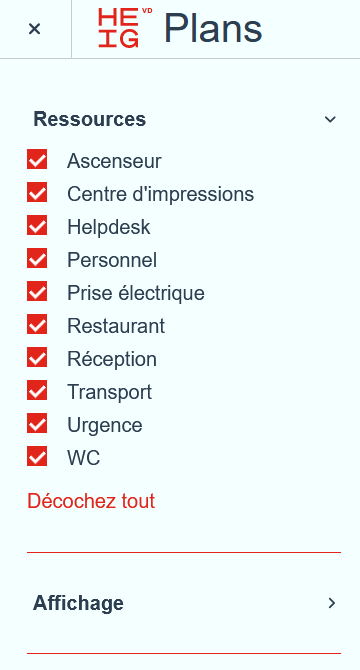
\includegraphics[scale=0.5]{frontend-filtresRessources.png}
    \caption{Outil de filtrage des ressources}
    \label{fig:ressources-filtre}
\end{figure}

L'outil de filtrage des ressources (voir figure \ref{fig:ressources-filtre}) se trouve dans le menu accessible à partir du bouton à gauche du header.
Il permet de sélectionner les types de ressources à afficher.
Si elle sont sélectionner les icones des ressources s'affichent sur le plan.
Dans le cas contraire les icones sont masqués.

Le design de l'outil est plus abouti que la conception initial : Les cases à cocher se trouvent à gauche, et
il se trouve dans un menu déroulant.

\subsubsection{Outil changement d'affichage}

\begin{figure}[h]
    \centering
    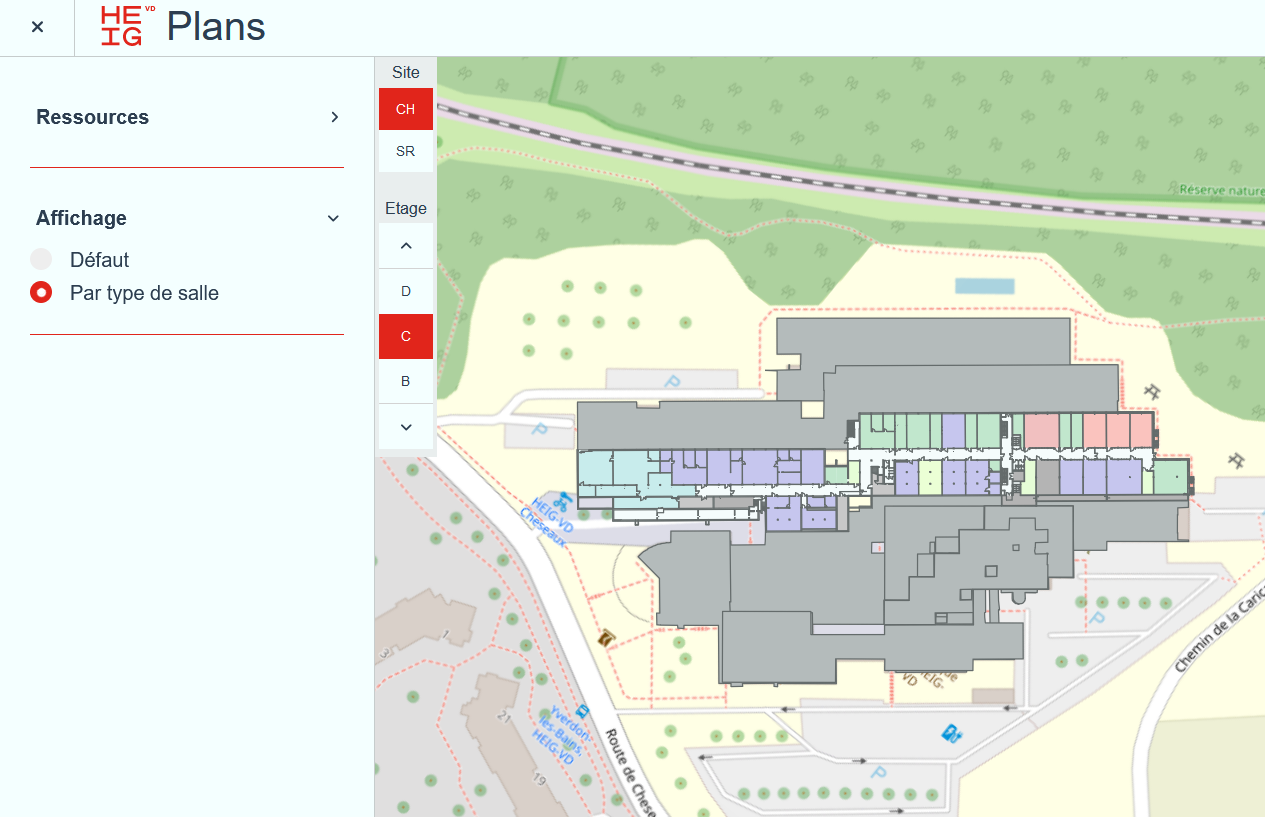
\includegraphics[scale=0.4]{frontend-affichageParType.png}
    \caption{Outil de changement d'affichage et effet sur le plan}
    \label{fig:affichage}
\end{figure}

L'outil de changement d'affichage (voir figure \ref{fig:affichage}) permet de modifier la présentation du plan.
Actuellement deux affichages différents sont disponible :
Celui par défaut et un affichage qui colorise les salles en fonction du type de salle.

Lors de la conception du design cet outil n'avait pas été planifié.

\subsubsection{Interraction avec le plan}
L'utilisateur peut interragir avec le plan en cliquant sur des salles ou des icones de ressources.
S'il le fait, celle-ci se met en mode sélectionné et l'application affiche la fenêtre d'information.

Cela est possible car \gls{ol} fournit des évènement lors de l'interraction avec le plan.

Grâce à \gls{ol} il est possible de sélectionner plusieurs salles ou ressources en maintenant la touche shift.
Ceci est géré par la fenêtre d'informations en affichant les infos de chaque salle ou ressource.

\subsubsection{Outil de recherche}

\begin{figure}[h]
    \centering
    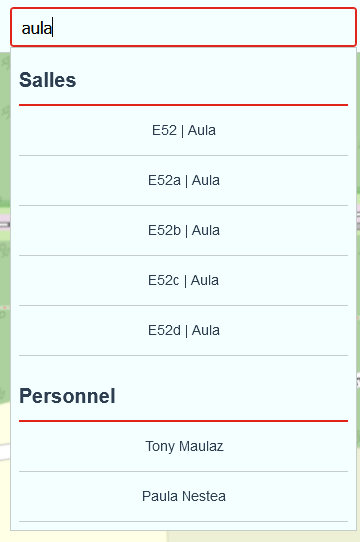
\includegraphics[scale=0.5]{frontend-recherche.png}
    \caption{Outil de recherche avec menu des suggestions}
    \label{fig:recherche}
\end{figure}


L'outil de recherche (voir figure \ref{fig:recherche}) permet de rechercher une salle pas son numéro ou son nom .
Il permet aussi de trouver la salle ou se trouve un collaborateur de l'école en écrivant son nom.

A partir de deux caractères écris, l'outil propose des suggestions contenant la chaîne de caractères de salle ou de collaborateur.
L'utilisateur peut cliquer sur une des suggestions.
S'il le fait, le plan change pour afficher la salle concerné en rouge et affiche les informations de celle-ci dans la fenêtre d'information.

Si l'outil n'as aucune suggestions à proposer. il affiche une erreur.
Si l'utilisateur clique sur une personne qui a une salle non implémenté dans la base de données,
un message d'alerte le précise à l'utilisateur.

Lorsque l'utilisateur clique en dehors de la barre de recherche, le menu de suggestions disparait,
et reapparait lorsqu'il reclique à l'intérieur.

Afin de limiter, les requêtes au serveur-api, les données des salles sont mis en cache à partir de deux caractères.
Ce cache est réinitialisé quand l'utilisateur clique sur une suggestion, ou qu'il efface sa saisie en dessous de deux caractères.

Le design de l'outil n'est pas très différent de la conception initiale : l'icone de loupe n'apparaît plus dans  la barre de recherche.
Les suggestions de salle propose en plus du numéro le nom de la salle.

\subsubsection{Fenêtre d'informations}

\begin{figure}[h]
    \centering
    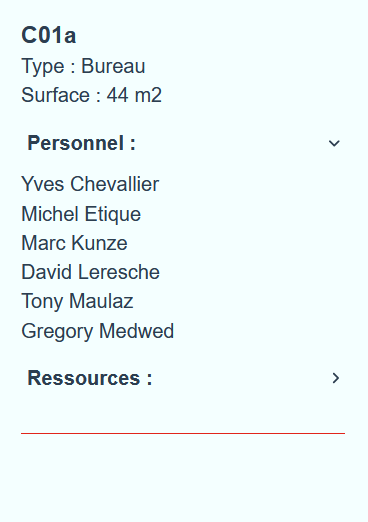
\includegraphics[scale=0.5]{frontend-info.png}
    \caption{Fenêtre d'informations}
    \label{fig:info}
\end{figure}

La fenêtre d'informations (voir figure \ref{fig:info}) peut apparaître soit après une recherche, soit loss d'une interraction avec le plan.
Celle-ci fait apparaître toutes les informations disponible de la salle ou de la ressource.
Dans le cas d'une salle, il peut afficher dans une liste déroulante la liste du personnel associé à celle-ci s'il y en a,
et la liste des ressources associé à celle-ci , s'il y en a.

Pour quitter la fenêtre d'information, il faut cliquer directement sur le plan.

\subsection{Responsivité}

\begin{figure}[h]
    \centering
    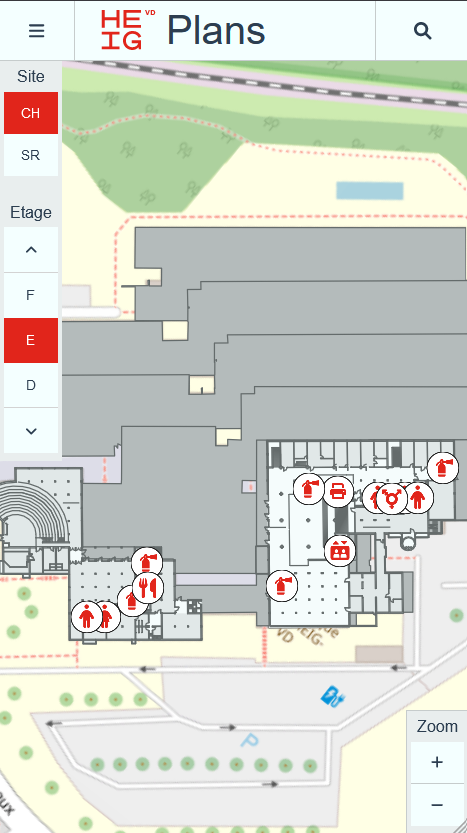
\includegraphics[scale=0.5]{frontend-responsive-portrait.png}
    \caption{Affichage sur smartphone en mode portrait}
\end{figure}

Afin de garantir l'accessibilité des fonctionnalités, lors de l'utilisation de l'application,
l'affichage s'adapte en fonction de la taille de l'écran.

Si la largeur de l'écran est trop petite, la barre de recherche deviens un bouton avec un icone de loupe.
Si l'utilisateur clique dessus, un menu de recherche le bouton de gauche, le logo et le titre de l'application
sont remplacés par une barre de recherche.
Celui redevient normale lorsque l'utilisateur reclique sur le bouton ou finalise sa recherche.

La fenêtre d'informations s'adapte aussi s'il la largeur est trop petite.
Il s'affiche sur le bas de l'écran au lieu de la droite.

Si la hauteur de l'écran est trop petite, le menu, comportant les outils de changement de bâtiment et d'étages,
se place sur deux colonnes.

\begin{figure}[h]
    \centering
    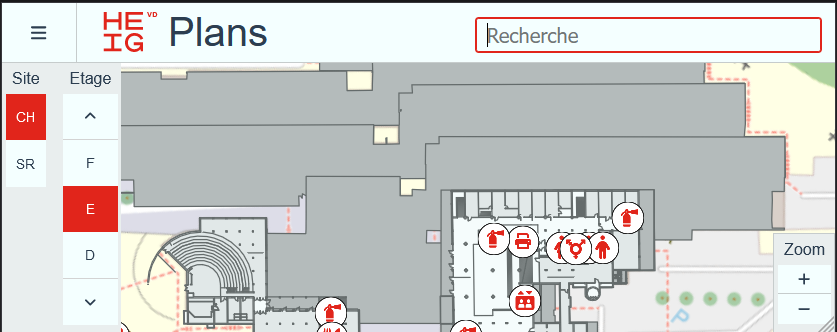
\includegraphics[scale=0.5]{frontend-responsive-paysage.png}
    \caption{Affichage sur smartphone en mode paysage}
\end{figure}

\section{Déploiement}

\subsection{Docker Compose}
Docker compose est une méthode proposé par \gls{docker} qui permets de Démarrer tous les containers de l'infrastructure en une seule commande à partir d'un fichier de configuration.
Ce fichier permet aussi de paramétrer chaque container et les communications entre ceux-ci.

\subsection{Déploiement sur la machine virtuelle}
Afin d'accueillir les différents container, il a fallu préparer la machine virtuelle en téléchargeant le logiciel docker.
Puis transférer le fichier de configuration pour docker compose, ainsi que les fichiers sql.
Il suffit ensuite de démarrer la construction des images, à l'aide du fichier de configuration.

Celui-ci va télécharger les 4 images nécéssaires pour la création des containers, soit \gls{traefik} le reverse-proxy,
\gls{postgis} la base de données et les images du serveur et du serveur-api préalablement créé et hebergé sur \gls{cicd}.
Il va par la suite créer les containers, les paramétrer et créer les liens pour la communication entre les containers.

Une fois fini, le site est mis à disposition de tous.

\subsubsection{Paramétrage \gls{postgis}}
Lors de la construction du container \gls{postgis}, les paramètres d'accès à la base de données sont définis.
La base de données va aussi être construite, avec ses tables, et les données remplissant ces tables en utilisant les fichiers SQL fourni.

\subsubsection{Paramétrage \gls{traefik}}
Lors de la construction du container \gls{traefik}, on va définir les points d'entrées auxquelles les clients accèdent aux serveurs,
ainsi que les règles permettant de diriger vers le bon serveur.

\subsubsection{Paramétrage serveur-api}
Lors de la construction du container serveur-api, le nom du container contenant la base de données,
ainsi que les paramètres pour y accéder lui sont précisés.

\chapter{Conclusion}

\section{Critique de la solution}

\subsection{Comparaison avec le cahier des charges}
Cette section compare le travail planifié par le cahier des charges avec le travail accompli.
Cette comparaison est résumé dans le tableau \ref{charge}.

\begin{table}[h]
    \begin{center}
        \begin{tabular}{l|l|l}
            Nom des tâches                     & Est nécéssaire & Etat d'avancement \\ \hline
            Visualisation plan Cheseaux        & Oui            & Complet           \\
            Affichage noms des salles          & Oui            & Complet           \\
            Affichage qualificatifs des salles & Oui            & Complet           \\
            Outil de changement d'étages       & Oui            & Complet           \\
            Surface des salles                 & Oui            & Complet           \\
            Responsive                         & Oui            & Complet           \\
            Hebergé sur une machine virtuelle  & Oui            & Complet           \\
            Comporte une base de données       & Oui            & Complet           \\
            Localisation des ressources        & Oui            & Complet           \\
            Outil de filtrage                  & Non            & Complet           \\
            Outil de recherche                 & Non            & Partiel
        \end{tabular}
        \caption{Etat d'avancement des fonctionnalités du cahier des charges \label{charge}}
    \end{center}
\end{table}

Les différentes fonctionnalités nécéssaire ont été implémenté au niveau du code et complétés dans ce projet.
Seul l'outil de recherche a une implémentation partiel car la recherche par des critères, autre que par le nom, est inexistente.
Il n'est pas exclu d'améliorer chaque fonctionnalité, lors de futures versions du projet.

D'autres fonctionnalités non prévu initialement par le cahier des charges ont été implémenté.
Elles sont présenté dans le tableau \ref{autres}

\begin{table}[h]
    \begin{center}
        \begin{tabular}{l|l}
            Nom des tâches                   & Etat d'avancement \\ \hline
            Page de chargement               & Complet           \\
            Outil de changement de bâtiments & Complet           \\
            Outil de changement d'affichage  & Partiel           \\
            Interraction avec le plan        & Complet
        \end{tabular}
        \caption{Etat d'avancement des fonctionnalités suppllémentaires  \label{autres}}
    \end{center}
\end{table}

L'outil de changement d'affichage n'est que partiellement implémenté, car il ne propose que deux types.
D'autres types d'affichages pourront être développé comme un présentant la vacance ou non des salles de cours à un horaire précis.

\subsection{Traitement et création des données géographiques}
Le traitement des données est suffisant pour une démonstration des capacités de l'application web,
mais pas assez précis pour une version définitive : le géoréférencement des plans des étages est différent
et souffre d'un léger décalage entre chaque étage.
Il faudrait utiliser un meilleur outil que l'extension Vector Bender.

Les autres données géographiques sont dépendant de ce premier géoréférencement et devront être refait.
De plus, de nombreuses données n'ont pas été créé, comme celle concernant les deux autres sites de l'école.

Ces erreurs sont dûs à une méconnaissance des logiciels et des techniques dans ce domaine.
Ce travail devra être confié à une personne plus compétente dans le domaine de la création de données géographiques.

\subsection{Design de l'application}
Le design de l'application est satisfaisant car il ne fait pas application inachevé au premier regard.
Des pratiques d'expérience utilisateur ont été implémenté afin d'offrir aux utilisateurs une facilité de prise en main.

Cependant le design et l'éxpérience utilisateur pourrait être àmélioré par une personne plus compétente dans ce domaine.

\subsection{Backend}
Le backend est simple et suffisant pour acheminer les données depuis la base de données.
C'est pourquoi il a été développé avec des technologies de base.
Cependant s'il fallait le complexifier, il faudrait envisager d'autres technologies comme le framework Nest JS.

\subsection{Frontend}
Le frontend est la partie la plus abouti du projet.
Les fonctionnalités nécéssaires et optionnels ont été implémenté.
Le code source a été séparé en plusieurs fichier afin d'offrir une compréhension du projet.
Les différentes fonctionnalités ont été testé.

Cependant, il contient sûrement des erreurs dûs à un manque d'expérience et de connaissances dans les bonnes pratiques à utiliser.

Les tests End-to-end servant servant à tester l'application n'ont pas été implémenté.
Il faudrait aussi faire tester l'application par une plus grande part d'utilisateurs afin de voir leur utilisations et detecter des bugs rares.

\section{Critique de la méthode de travail}

\subsection{Critique du temps accrédité au projet}
Ce projet n'atteint pas les 450 heures prévus, et accuse un manque de XX heures.
Cela est dû à plusieurs facteurs :

\begin{itemize}
    \item Démarrage lent du projet, lors de la récupération d'informations.  (8 heures)
    \item Une semaine n'as pas pu être mise à contribution à cause d'une semaine spéciale (Crunch) prévu par l'école. (12 heures)
    \item Une semaine a été perdu à cause de maladie. (12 heures)
    \item D'autres petits projets ont pris du temps sur celui-ci en fin de semestre. (12 heures)
    \item 6 jours d'indisponibilté à la fin du projet. (48 heures)
\end{itemize}

Une semaine d'extension a été accordé à l'accomplissement du projet, récupérant 40 heures.

En tout, environ 52 heures ont été perdu. XX ont pu être rattrapés, mais pas l'intégralité.

Certains points, comme la maladie, pourrait être comptabilisé comme imprévus et ferait parti des 90 heures planifié.

Malgré les retards, toutes les fonctionnalités prévus ainsi que d'autres ont été implémenté.
Aucune autres aurait été développé lors de ce projet.
Ce temps aurait plutôt été consacré dans l'optimisation des existentes, l'implémentation de tests end to end et de performances et la correction de bugs.

\subsection{Comparaison entre plannification et réalisation}


\section{Implémentation futures}
Ce projet peut être étendu de plusieurs manières.
D'abord en améliorant les différentes fonctionnalités implémenté dans cette solution.
De plus, on peut implémenter les fonctionnalités suivantes :

\begin{itemize}
    \item Recherche par critère.
    \item Affichage de la vacance des salles de cours.
    \item Outil d'exportation et d'impression du plan.
    \item Outil de plus court itinéraire vers une ressource ou une salle.
    \item Outil de dessin vectoriel sur le plan.
    \item Outil de rajout de ressources localisé pour les administrateurs de l'application.
    \item Localisation de l'utilisateur sur le plan.
    \item Technologie pour monitorer le traffic de l'application.
    \item Optimiser la détection par les moteurs de recherches.
\end{itemize}

Cette liste est loin d'être exaustive.

\section{Conclusion personnel}
Le travail accompli est, à mon avis, bon. Il est perfectible sur de nombreux points
et le temps mis à disposition n'est pas suffisant,
pour autant, c'est le travail d'une seule personne, ne connaissant,au départ, que peu de choses dans le domaine des \gls{websig}.

Un tel projet, pour être finalisé, devrait soit être réalisé par une équipe de différents corps de métier,
soit plannifier une période de temps plus grande pour un apprentissage plus approfondi des différents domaines.

\vfil
\hspace{8cm}\makeatletter\@author\makeatother\par
\hspace{8cm}\begin{minipage}{5cm}
    %%if
    % Place pour signature numérique
    \printsignature
    %%fi
\end{minipage}
\clearpage

\appendix
\appendixpage
\addappheadtotoc

\chapter{Planning}

\begin{figure}[H]
    \centering
    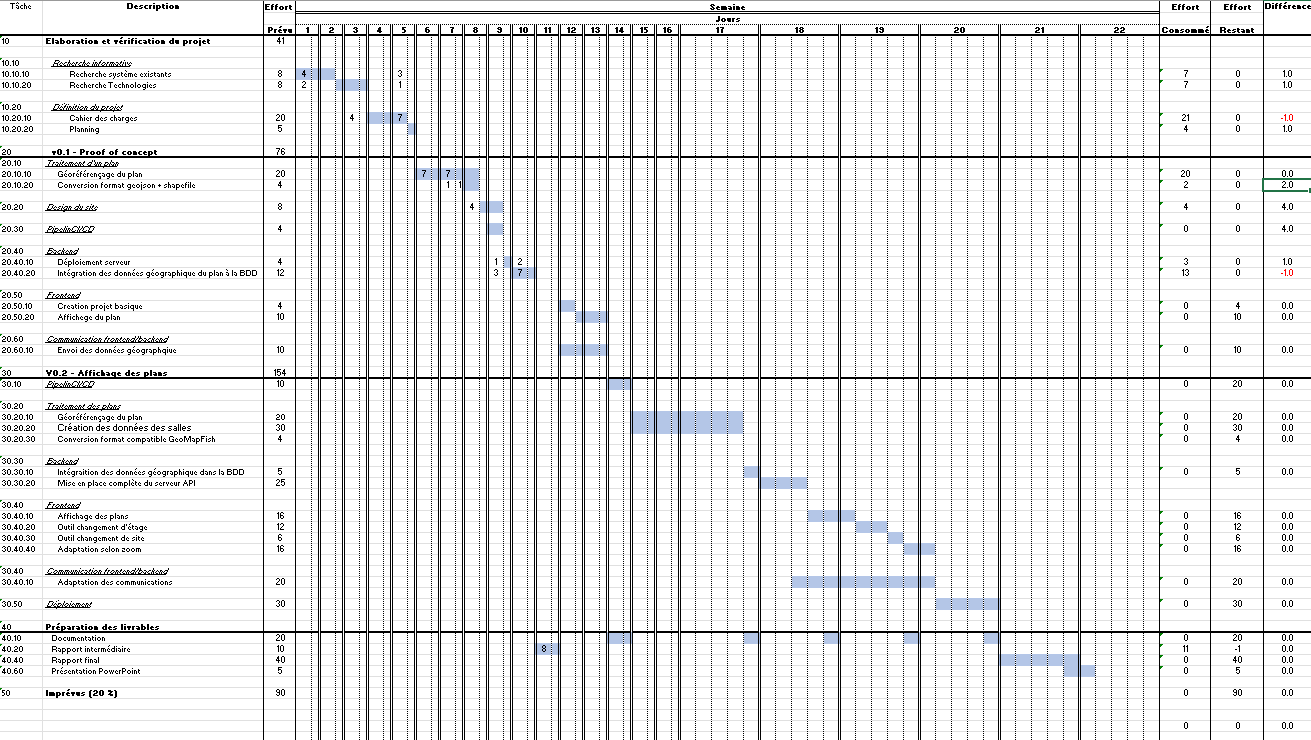
\includegraphics[scale=0.6, angle=90]{planning.png}
\end{figure}

\let\cleardoublepage\clearpage
\backmatter

\label{glossaire}
\printnoidxglossary
\printbibliography
\label{index}
\printindex

\end{document}
